\documentclass[10pt,twocolumn,letterpaper]{article}
\usepackage[square,sort,comma,numbers]{natbib}
\usepackage{cvpr}
\usepackage{times}
\usepackage{epsfig}
\usepackage{graphicx}
\usepackage{amsmath}
\usepackage{amssymb}
\usepackage{natbib}
\usepackage{color}
\usepackage{subcaption}
\usepackage{float}

% Include other packages here, before hyperref.

% If you comment hyperref and then uncomment it, you should delete
% egpaper.aux before re-running latex.  (Or just hit 'q' on the first latex
% run, let it finish, and you should be clear).
\usepackage[breaklinks=true,bookmarks=false]{hyperref}

\cvprfinalcopy % *** Uncomment this line for the final submission

\def\cvprPaperID{67} % *** Enter the CVPR Paper ID here
\def\httilde{\mbox{\tt\raisebox{-.5ex}{\symbol{126}}}}

% Pages are numbered in submission mode, and unnumbered in camera-ready
%\ifcvprfinal\pagestyle{empty}\fi
\setcounter{page}{4321}
\begin{document}

%%%%%%%%% TITLE
%\title{New Tricks for Single-Image Super-resolution}
\title{New Techniques for Preserving Global Structure and Denoising with Low Information Loss in Single-Image Super-Resolution}
%: Denoising While Upsampling and Preserving Large-Scale Structure}

% \author{Alex Damian\\
% {\tt\small ad315@duke.edu}
% % For a paper whose authors are all at the same institution,
% % omit the following lines up until the closing ``}''.
% % Additional authors and addresses can be added with ``\and'',
% % just like the second author.
% % To save space, use either the email address or home page, not both
% \and
% McCourt Hu \\
% {\tt\small secondauthor@i2.org}
% \and
% Nikhil Ravi \\
% {\tt\small secondauthor@i2.org}
% \and
% Sachit Menon \\
% {\tt\small secondauthor@i2.org}
% \and
% Webster Bei \\
% {\tt\small secondauthor@i2.org}
% }

\author{Yijie Bei \and \hspace*{-5pt} 
Alex Damian \and \hspace*{-5pt} 
Shijia Hu \and \hspace*{-5pt} 
Sachit Menon \and \hspace*{-5pt} 
Nikhil Ravi \and \hspace*{-5pt} 
Cynthia Rudin\thanks{All authors contributed equally. Thanks to other members of Duke Data Science Team} \and Duke University}

%.}\\\vspace*{5pt}
%{\mbox{Duke University}}\hspace*{00pt}}

\maketitle
%\thispagestyle{empty}

%%%%%%%%% ABSTRACT
\begin{abstract}
  This work identifies and addresses two important technical challenges in single-image super-resolution: (1) how to upsample an image without magnifying noise and (2) how to preserve large scale structure when upsampling. We summarize the techniques we developed for our second place entry in Track 1 (Bicubic Downsampling), seventh place entry in Track 2 (Realistic Adverse Conditions), and seventh place entry in Track 3 (Realistic difficult) in the 2018 NTIRE Super-Resolution Challenge. Furthermore, we present new neural network architectures that specifically address the two challenges listed above: denoising and preservation of large-scale structure. 
\end{abstract}

%%%%%%%%% BODY TEXT
\section{Introduction}
Super-resolution (SR) is a classic problem in image processing where the goal is to generate a high resolution image from one or more low resolution images. Applications of super-resolution are wide-ranging. For instance, SR is important for allowing modern high-definition displays to function properly when showing video recorded at lower resolutions. SR also has many applications in medical imaging, such as reducing noise in images stemming from uncontrollable patient motions \cite{Robinson1}. This work focuses on single image super-resolution, which is useful for photographic enhancement, license plate recognition, satellite imaging, and other remote sensing applications such as recognition of a military target \cite{Yue2}. 

Deep learning techniques can learn a mapping directly from low resolution to high resolution images, where all feature construction is automated. This makes some types of complex preprocessing much easier than previous approaches, for example, we no longer need to explicitly choose a dictionary of low-level features (e.g., edge detectors) to convolve with the image. The fact that training deep neural networks has become much easier within the past few years has led to more reliable automated training. On the other hand, the fact that these deep learning methods use recursive mathematical formulas that are now much more complicated than before makes it more difficult to determine how to best troubleshoot them to achieve higher-quality performance.

In this work we discuss several insights into the problem of single-image super-resolution -- many of which have led to higher quality performance beyond entries from last year's NTIRE single-image SR competition. These insights concern the amplification of noise when upsampling and the preservation of large scale structure in enhanced images. We introduce neural network architectures for both the denoising problem (DeNoising for Super-Resolution -- DNSR) and the problem of preserving large-scales structure (Automated Decomposition and Reconstruction for Super-Resolution -- ADRSR). Additionally we present a set of tricks that provided boosts in SR performance. 

For denoising while upsampling, we present the DNSR (and more basic DNISR) architecture that concatenates two networks, where the first network is for denoising and the second is a baseline method for SR. This leverages domain knowledge that the noise should not have been in the low-resolution image in the first place and thus we should not amplify it.
Training these concatenated networks led to improvements in performance in Track 2 (realistic mild adverse conditions) and Track 3 (realistic difficult) of the NTIRE SR 2018 challenge. 

Modern methods for SR have trouble preserving large scale structure. Even if the high resolution images look realistic in local patches, the global structure (such as stripes that reach across the full image) can have serious visible faults. We present an architecture for preserving structure at multiple scales. In our network, ADRSR, the original image is downsampled multiple times, convolutions are performed on each of the downsampled images, and combined to form the final high-resolution image. This allows a multiscale reconstruction of the image that includes information about the larger scales before modeling information at the smaller scales.

%Our ideas about denoising leverage the fact that we understand the generative process for the noise, which is often known in real applications based on the type of camera that took the picture or on the type of noise typical in, for instance, various kinds of medical imaging applications. In the case of the NTIRE SR challenge, in Track 1 the images were created from bicubic downsampling, whereas in Track 2, gaussian noise was also added to the images. Finding ways to incorporate our knowledge about the noise into the algorithm’s input led directly to better SR performance. Our ideas can be built onto the baseline deep learning algorithm that we used for training, which was last year’s winning entry.

The architectures for denoising and preserving large-scale structure can be used with any network blocks used for SR; we used convolutional blocks from EDSR \cite{EDSR} within our implementations, but these can be changed to any other blocks. DNISR or DNSR combine any network for denoising with any network for SR. 
%The architecture used for preserving large-scale structure (ADRSR) can use any building blocks within in the convolutional layers. 

Most of the ideas discussed here were not implemented in time for the NTIRE 2018 SR competition deadline. However, we present a set of tricks that were helpful in achieving higher level performance during the competition. For instance, an idea used in our Track 1 (classic bicubic downsampling) entry was to randomly shuffle the red, green, and blue layers of the image during training, which helps as a form of self-ensembling. We also discuss different upsampling techniques, and find that for x8 amplification, we should learn the fully amplified image directly, because learning a x4 followed by a x2 amplification tend to lead to the spurious addition of details that do not exist in the original high-resolution image. 
 
All of these ideas were developed over the course of approximately 8 weeks by a team of 5 undergraduates with no previous experience in image processing.

Our entries in the 2018 NTIRE superresolution competition \cite{Timofte_2018_CVPR_Workshops} achieved seventh place in Track 2 (realistic mild adverse conditions), seventh place in Track 3 (realistic difficult) and second place in Track 1 (classic bicubic downsampling). 
\begin{table}[ht]
    \centering
    \begin{tabular}{c|c|c|c}
         & Track 1 & Track 2 & Track 3\\ \hline
         PSNR & 25.433 & 23.374 & 21.658\\
         SSIM & 0.7067 & 0.6252 & 0.5400
    \end{tabular}
    \caption{Competition Result}
    \label{tab:my_label}
\end{table}

\section{Previous Work}
Many approaches to single-image super-resolution are based on different methods of image upsampling. In particular, nearest-neighbors upsampling (in which each unknown pixel in the upsampled image is assigned the value of its nearest known neighbor) and bicubic upsampling (in which each unknown pixel in the upsampled image is assigned a value interpolated from its nearest known neighbors) are popular methods for basic upsampling \cite{babu2011survey,gilman2006near}. These methods, while simple and computationally efficient, do not provide realistic high-resolution images. More advanced methods attempt to build a map between low resolution images and high resolution images through a variety of different techniques. Some techniques include frequency-domain methods such as alias removal \cite{tsai1984multiframe}, recursive least squares \cite{kim1990recursive}, and multichannel sampling theorem methods \cite{ur1992improved}, as well as spatial-domain methods, such as iterated back-projection \cite{irani1993motion}, joint MAP restoration \cite{hardie1997joint}, and adaptive filtering \cite{patti1998new}.

%Among spatial-domain methods, example-based machine learning methods have recently come under scrutiny with the successes of 
Neural networks have recently been successful for image processing tasks, and through application of classical ResNet architectures, Ledig et al$.$  created one successful example of a convolutional neural network for super-resolution, called SRResNet \cite{LEDIG}. Their work showed that the use of residual blocks improved performance on super-resolution tasks over more traditional convolutional neural network architectures, and has become the basis for many future architectures for super-resolution. Lim et al$.$ then improved on this with their EDSR method by removing batch normalization, using an L1 rather than L2 loss function, and adding depth to the network \cite{EDSR}. While these models have seen some success in the super-resolution task for `clean' images (that is, images that have been bicubically downscaled with no further degradations), they do not show good results for images with noise, blur, or other degradations. 

A few recent interesting super-resolution techniques have been suggested for degraded images. Zhang et al$.$ \cite{IRCNN} suggested using CNN denoisers as a modular part of model-based optimization methods to perform various computer vision tasks including super resolution. Shocher et al$.$ \cite{zssr} proposed an unsupervised approach that trains an image-specific CNN at test time that learns to use the repetitive structure of images to fill in details where there previously were none.
%but this significantly increases the amount of time needed to process each image.

Other neural-network based methods, such as generative adversarial networks \cite{LEDIG}, have shown success in super-resolution as measured by human viewers. However, these networks achieve visual effects suitable for human viewing by `hallucinating' features from the low resolution image that are not necessarily in the original image, but would be believable given the low resolution image. As such, they are not as well suited for tasks that maximize similarity to the original high resolution image, such as PSNR and SSIM.

The methods introduced into this work are different in that they heavily leverage prior knowledge: DNSR leverages the knowledge that denoising before upsampling is helpful, while ADRSR uses a pyramid of downsampled images to borrow information at broader scales. The ideas within ADRSR and DNSR can be combined with any neural network approaches to denoising and super-resolution in order to include domain knowledge.

%One component of our contribution aims to improve objective-measure super-resolution for degraded images without training image-specific CNNs. 


%%%%%%%%%%%%%%%%%%%%%%%%%%%%%%%%%%%%%%%%%


\section{Challenges}
When approaching all three super-resolution tracks (corresponding to non-noisy and noisy images), we encountered multiple challenges.

First, there were challenges that were specific to the competition itself. One such challenge was that of \textit{model validation}, because the PSNR values of our algorithm varied wildly between images (see Figure \ref{fig:varyingpsnr}). Depending on which 100-image subset we used for validation, average PSNR values ranged from 22 to 27. This made it difficult to compare our results to others' and required us to fix a validation set of 100 images throughout training.

\begin{figure}[ht!]
    \centering
    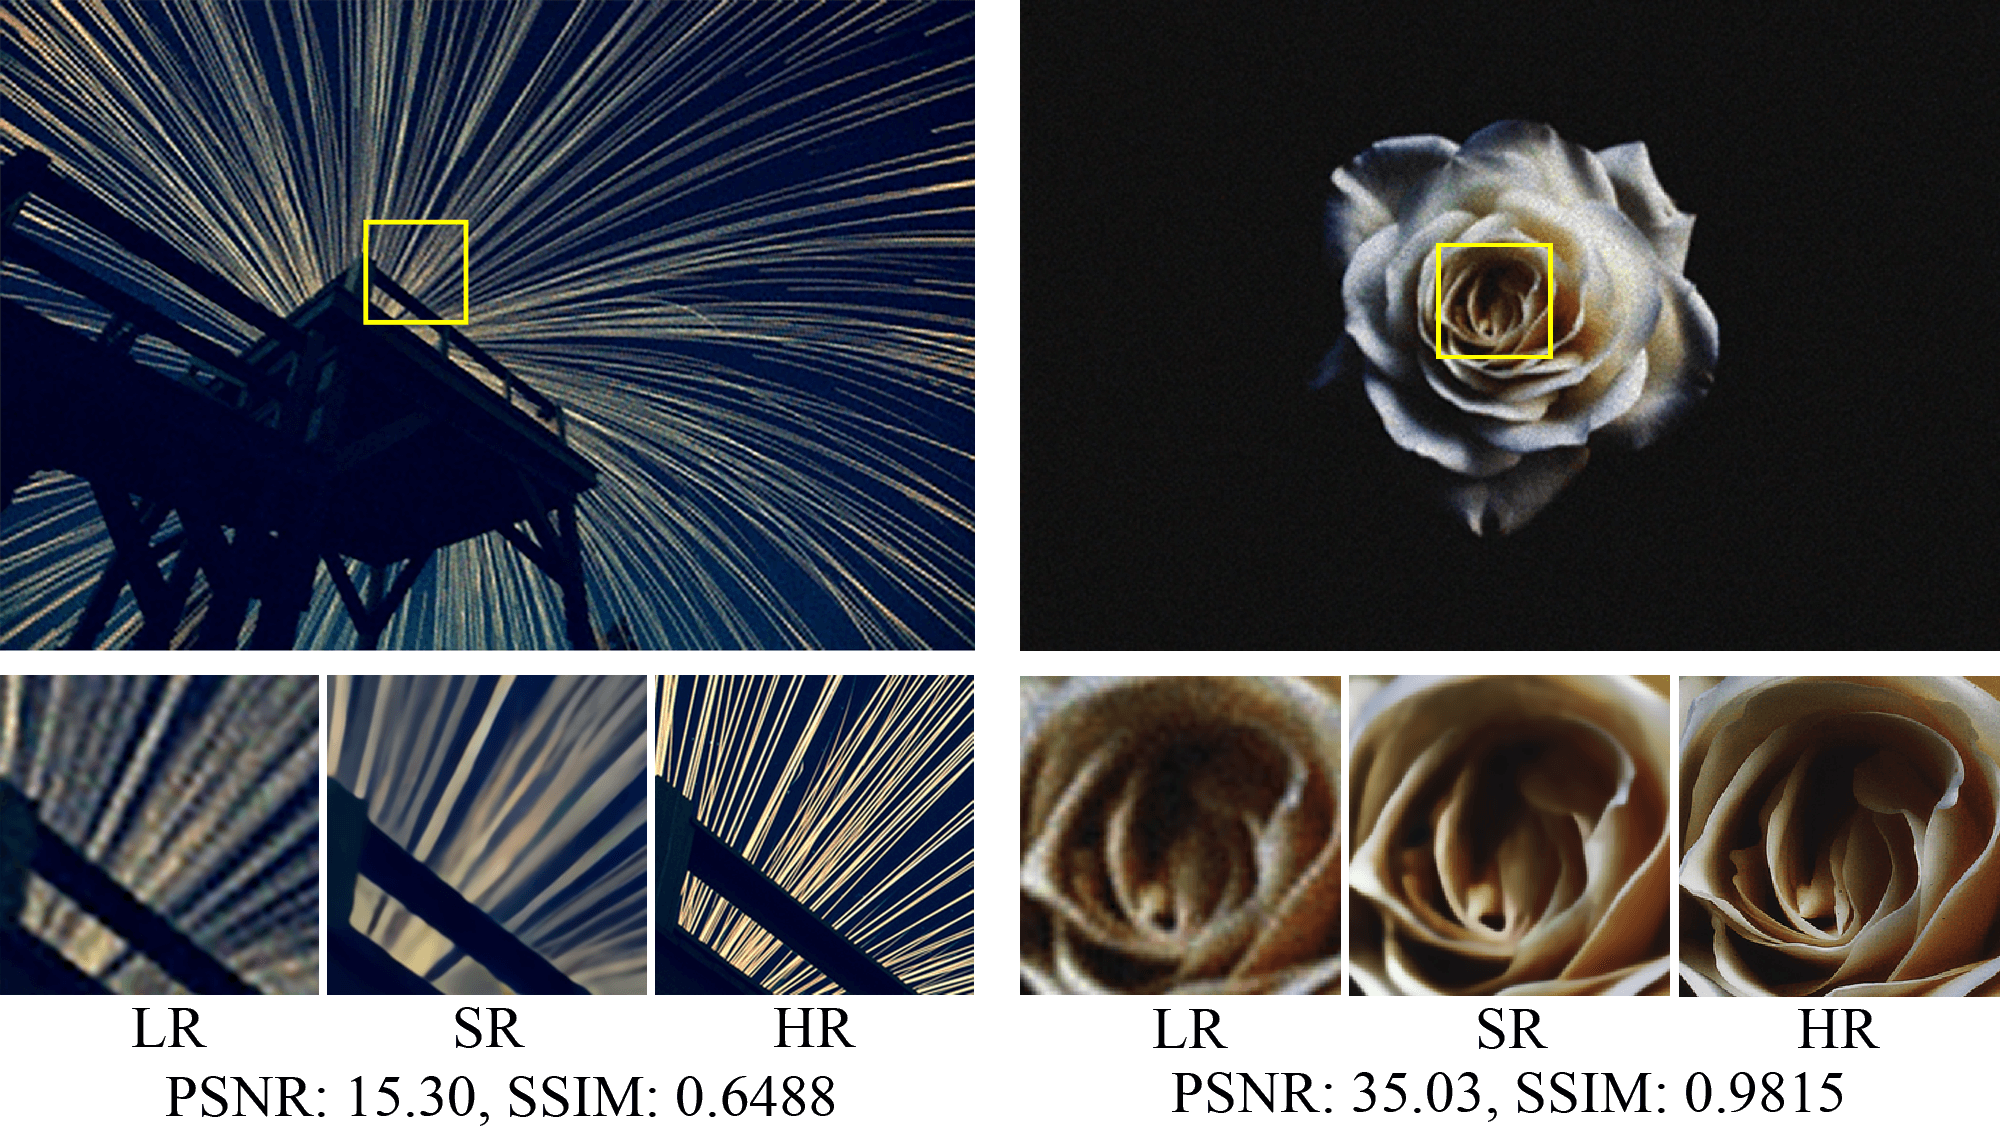
\includegraphics[width=\columnwidth]{Images/PSNR.png}
    \caption{Varying PSNR between our algorithm's images for Track 2}
    \label{fig:varyingpsnr}
\end{figure}

Particularly for noisy images, it is very difficult to avoid \textit{amplifying the noise while upsampling}. Several of the techniques we introduce here were useful for this, particularly the denoising and upsampling network DNSR for Tracks 2 and 3. Even without noise, artifacts tend to appear when upsampling by a factor of eight.



%\textbf{(Track 1)} Upsampler Error: When performing upscaling by a factor of $8$, the upsampler is much more important. (discussion of images, various upsampling methods)

%\item \textbf{(Track 1)} Memory Issues: Because we were upscaling with a factor of $8$, we could not train on $48\times 48$ low resolution patches (that would be super-upscaled to $384\times x384$ patches) without reducing the batch size, due to memory constraints.
%\item \textbf{(Track 2)} The Dataset: The given low resolution - high resolution pairs were misaligned, which hindered training. In addition, there was a difference in the overall brightness of the images. Therefore to preprocess the images, we aligned them, cropped the part of the images in common, and mean shifted them.

Most traditional denoisers require some knowledge of the noise itself, normally the standard deviation. To use any of these denoisers, it was imperative to \textit{reverse engineer} the noise. We took approximately flat areas of various images and considered the difference between the degraded low resolution images and down-scaled versions of the high resolution images. Because a blur kernel has no effect on flat regions of an image, this difference should be a good approximation of the noise (see Figure \ref{fig:hist}).
\begin{figure}
    \centering
    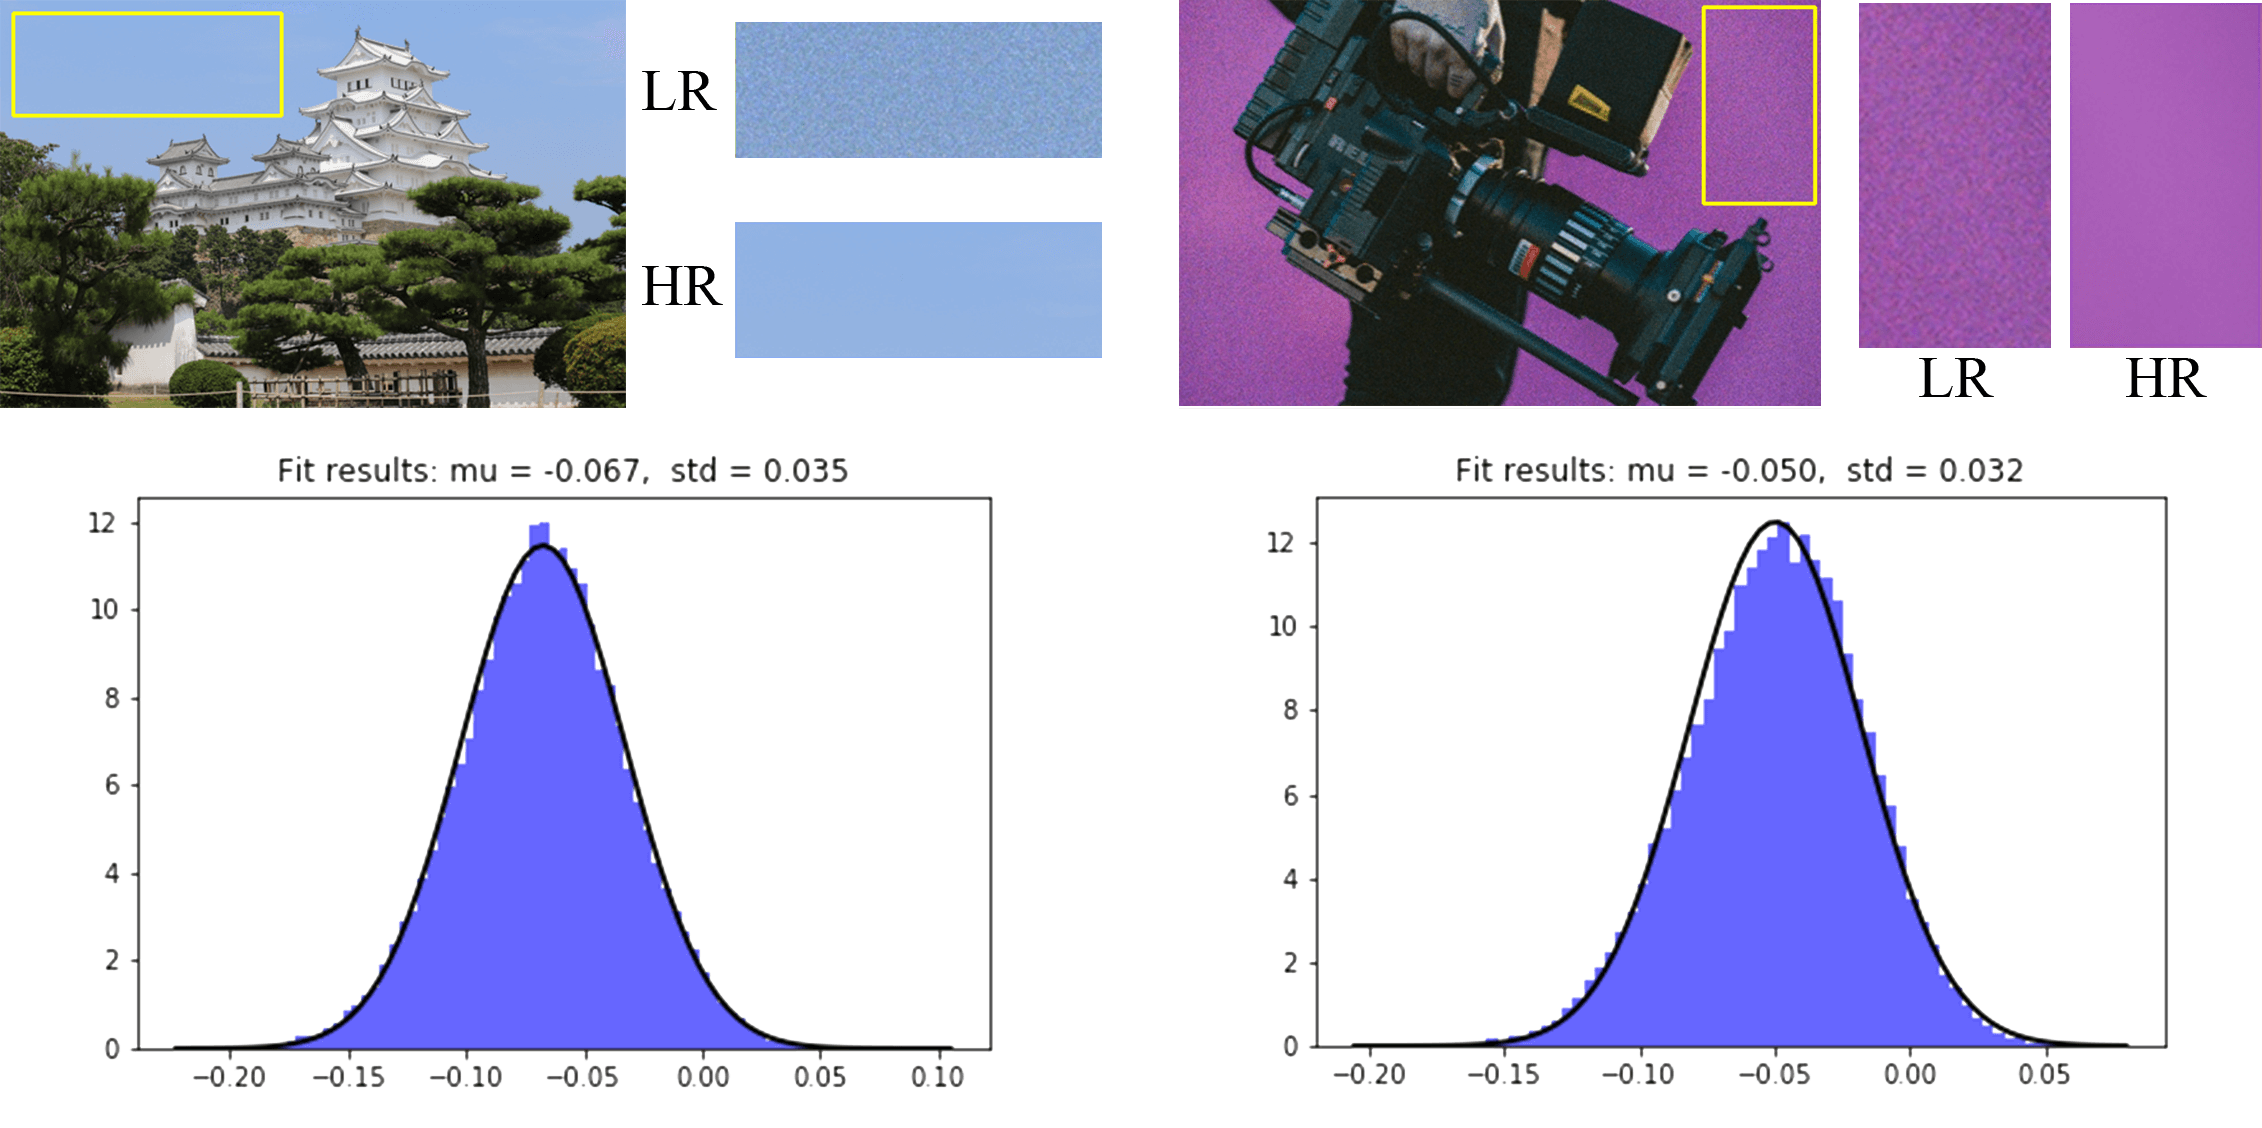
\includegraphics[width=\columnwidth]{Images/NOISE.png}
    \caption{Histogram of noise from two images}
    \label{fig:hist}
\end{figure}

%\item \textbf{(Track 2)} Incorporating Domain Knowledge: When picking our approach, we needed to pick a model that would allow us to incorporate our knowledge of the noise in a meaningful way.

Most prior convolutional networks for super-resolution tend to focus on increasing the resolution in local areas; however, this approach does not \textit{take into account more global patterns} (such as zebra stripes). Some recent work \cite{upanddown,zssr} have aimed to solve this problem in other promising ways, and we present a new method for handling this (ADRSR) in what follows.


%%%%%%%%%%%%%%%%%

%\section{Two New Types of Architecture for Superresolution}
%The first type of architecture we introduce, called ??, can discern global image features, and incorporate them in the final result. The second type of architecture specifically addresses denoising while upsampling, without losing too much information.


\section{ADRSR: A type of architecture that preserves global structure}

Figure \ref{fig:antialias} shows the types of problems that can arise from EDSR and similar SR algorithms. These algorithms consider local image patches, and do not aim to reconcile them with larger-scale patterns that crosscut into different patches.
Both increasing the depth of the network and increasing the size of each kernel allows the network to include larger scale patterns. However, these approaches are either hard to train, or do not converge at all. Thus, we reasoned that these larger patterns could be detected even by using a smaller kernel on a downsampled image without significant loss of information; the flexibility afforded by a large number of larger kernels may be unnecessary to capture this information.

The architecture that we introduce for preserving global structure is presented in Figure \ref{fig:multscalenet}, called Automated Decomposition and Reconstruction for SR (ADRSR). The original image is downsampled several times, with each downsampled image being fed through a parallel super-resolution network. This pyramid representation for the input allows us to create filters that capture patterns from the original image at various scales. We then iteratively combine the information from the various upscaled images to produce a final, more accurate image that respects global structure. When running the network forward on a new image, it would start from the coarsest scale, and iteratively add more detail on the finer scales. 

In Figure \ref{fig:multscalenet}, the SR network labeled in the figure can be replaced with any SR network. 

\begin{figure*}[ht!]
\centering
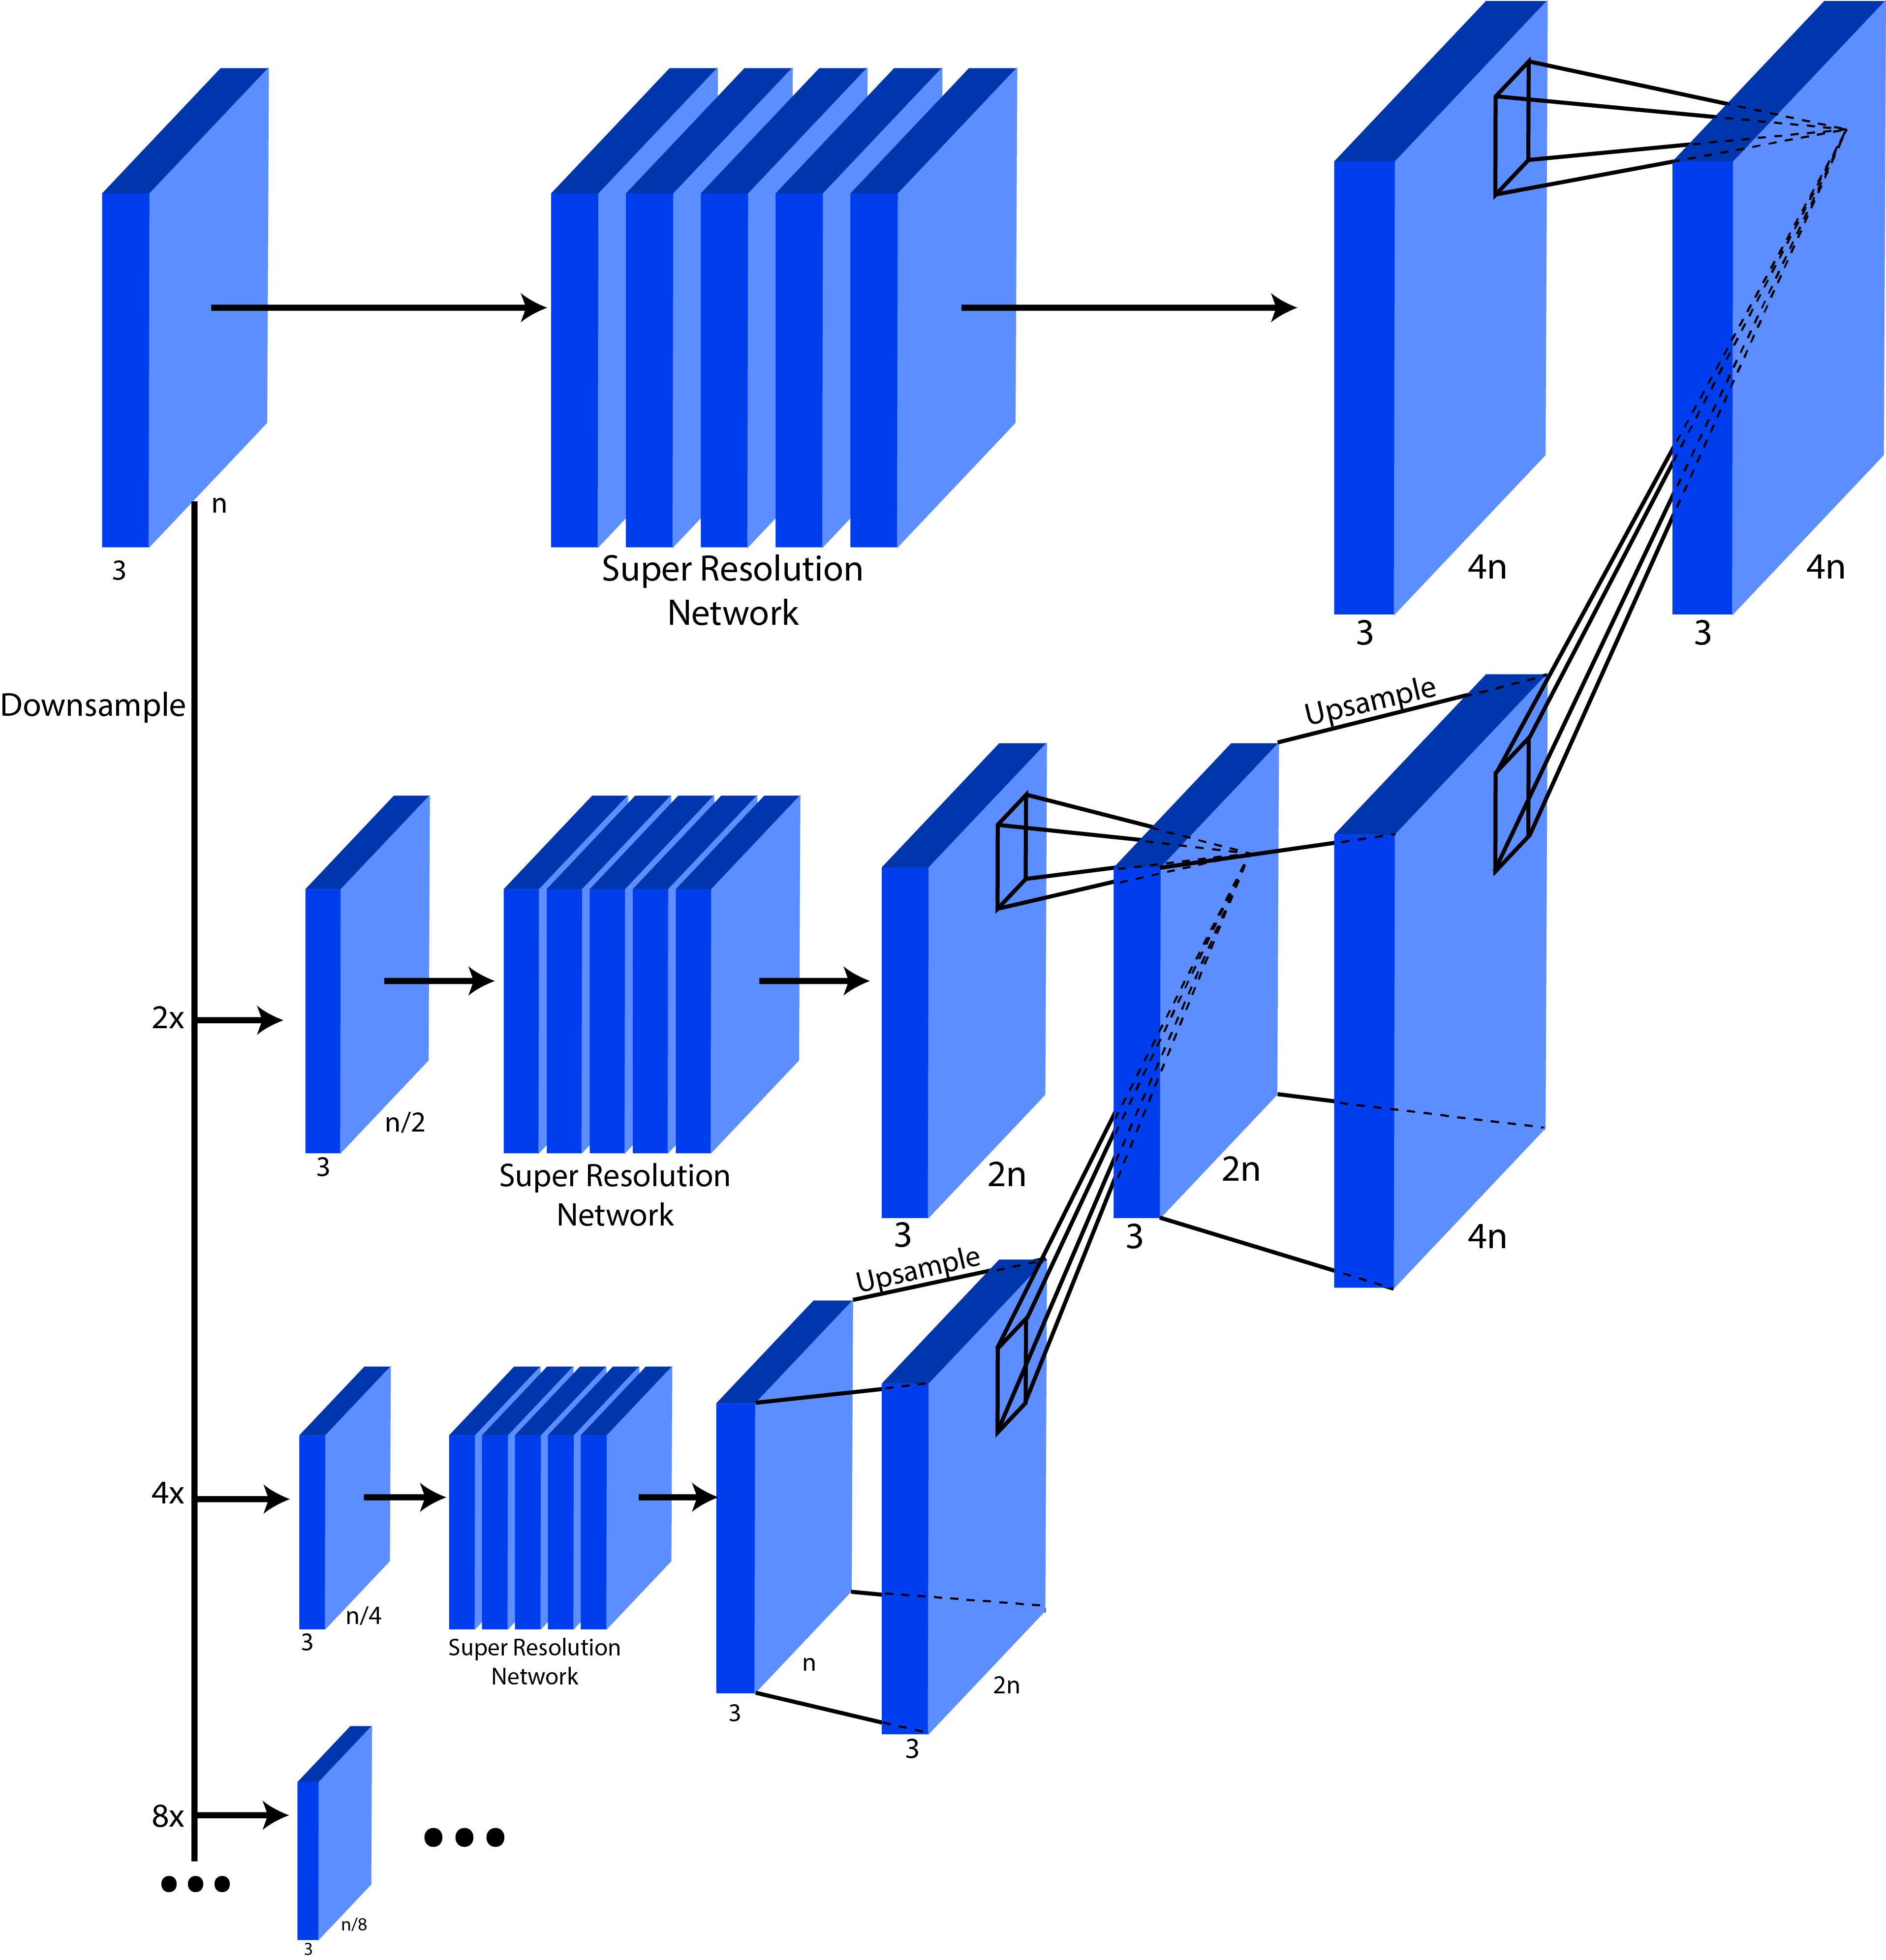
\includegraphics[width=0.70\textwidth]{Images/MultipleScaleNet.png}
\caption{ADRSR Network with a x4 super resolution network
\label{fig:multscalenet}}
\end{figure*}

We trained ADRSR to perform x8 upscaling using a baseline EDSR upscaler as the modular super resolution network. We initialized the bottom copy of EDSR with our fully trained baseline model, and then iteratively trained each successive level by temporarily removing all levels above it, and directly outputting the final result of that level (see Figure \ref{fig:multscalenet}). While training a level, we froze all weights except for those in the super resolution network in that level and the weights of the convolutional layer that combines the results of the current level with the result from the previous level. After training each level to convergence, we unfroze all of the weights and trained the entire network at once, which eliminated some blocky artifacts that appeared as a result of the upscaling process (see Figure \ref{fig:blockyup}). The results of this can be seen in Table \ref{tbl:adrsr} and Figure \ref{fig:adrsr}.

\begin{table}[ht!]
    \centering
    \begin{tabular}{c|c|c}
       \footnotesize{Algorithm}  & \footnotesize{EDSR} & \footnotesize{ADRSR}\\ \hline
        \footnotesize{PNSR} & \textcolor{red}{25.49} & 25.38\\
        \footnotesize{SSIM} & \textcolor{red}{0.6930} & 0.6898\\
    \end{tabular}
    \caption{Comparison of ADRSR to baseline EDSR
    \label{tbl:adrsr}}
\end{table}

\begin{figure}[htbp]
	    \centering
	    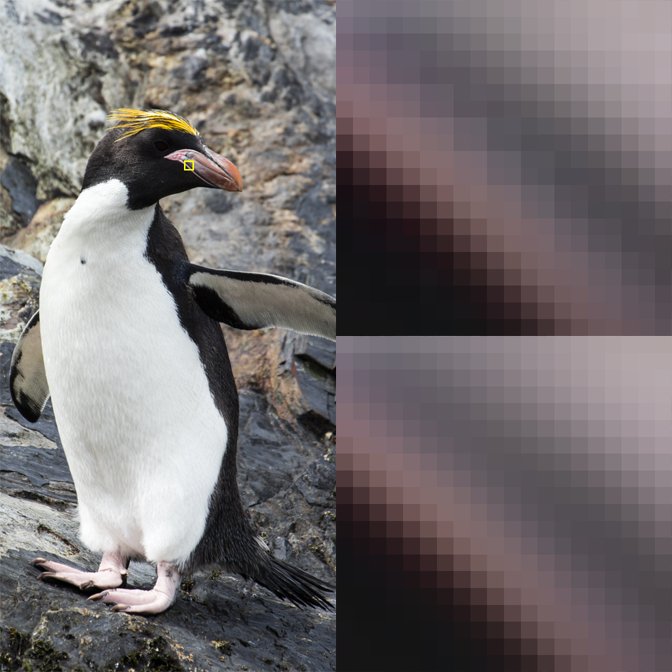
\includegraphics[width=\columnwidth]{Images/blockyup.png}
	    \caption{Before unfreezing all of the weights, ADRSR tended to produce blocky artifacts (top-right), however after unfreezing all of the weights and training for a few more epochs, the artifacts disappeared (bottom-right).}
	    \label{fig:blockyup}
\end{figure}

\begin{figure*}[ht!]
    \centering
    
    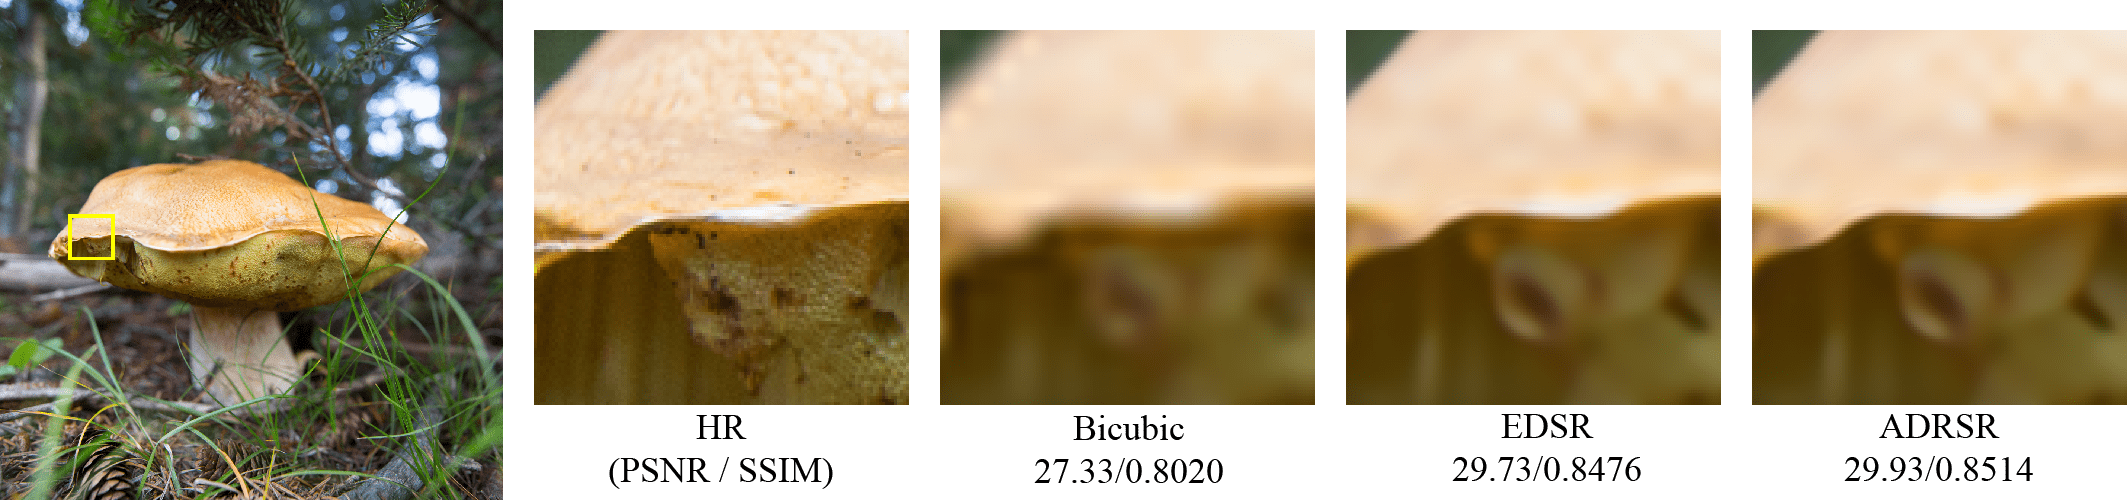
\includegraphics[width=\textwidth]{Images/Samples/3-1.png}\\
    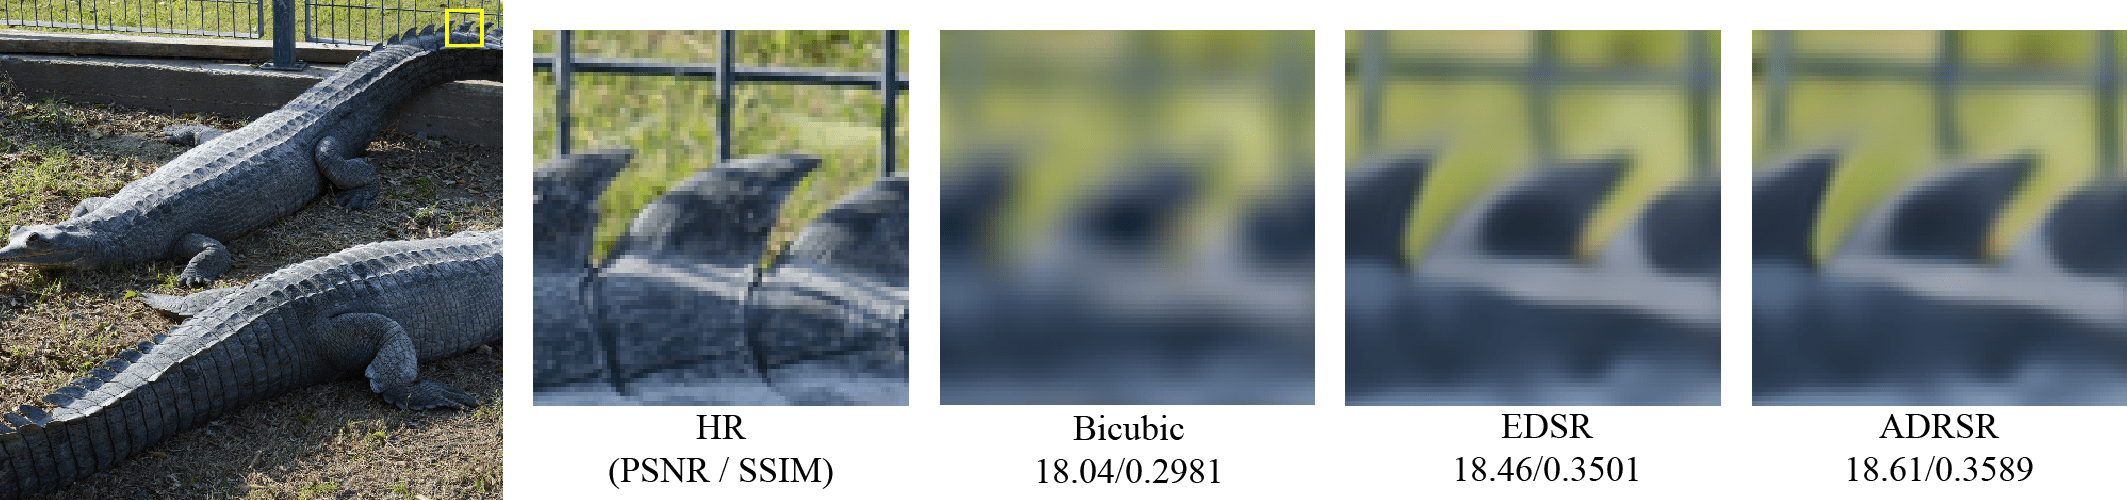
\includegraphics[width=\textwidth]{Images/Samples/3-2.png}\\
    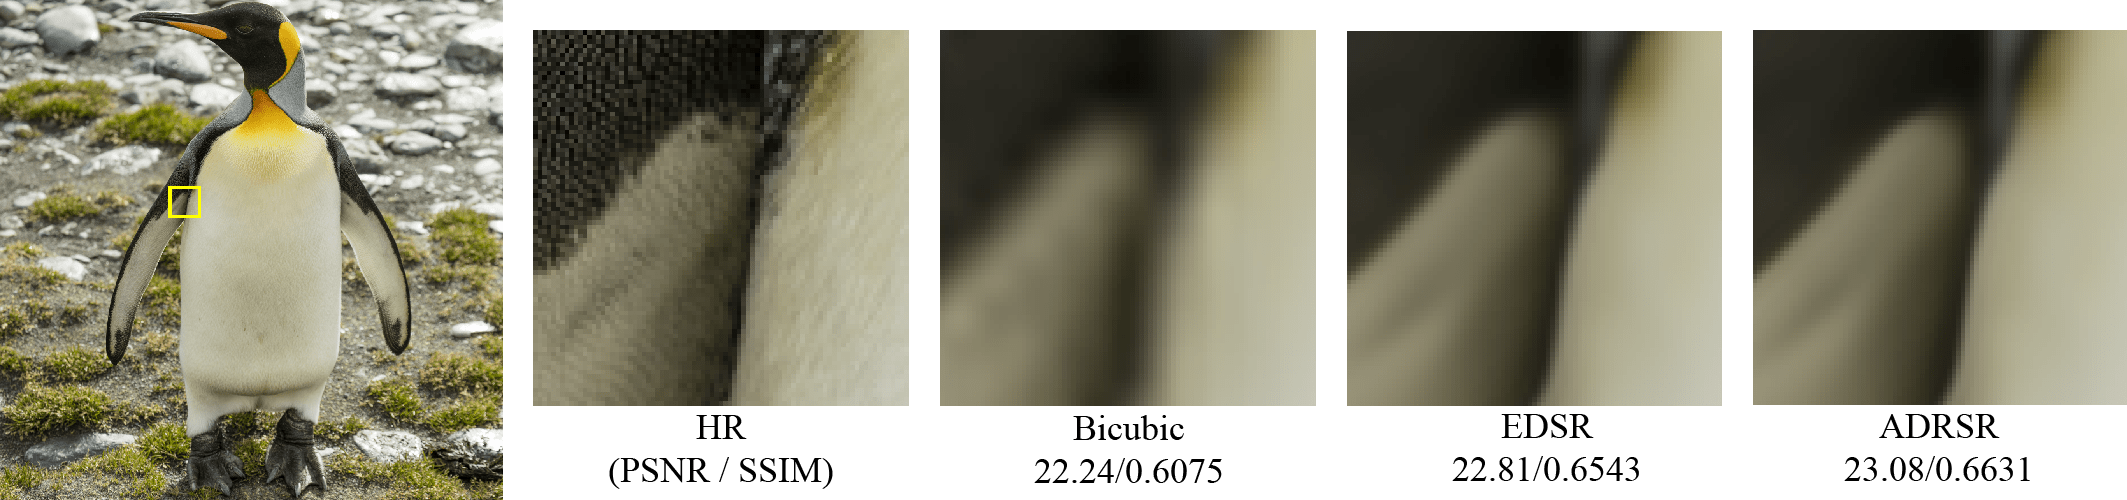
\includegraphics[width=\textwidth]{Images/Samples/3-3.png}
    
    \caption{Comparison of baseline EDSR with ADRSR. Although the PSNR values of EDSR and ADRSR are similar, ADRSR tends to produce sharper lines and edges throughout the validation set.}
    \label{fig:adrsr}
\end{figure*}

While the results do not show any difference from EDSR in terms of numerical performance metrics, the network's multiscale reconstruction was intuitive and interesting. It is possible that this architecture could be useful for other applications besides PSNR/SSIM optimization.

%%%%%%%%%%%%%% DNSR section

\section{DNSR: A type of architecture for denoising with low information loss for SR}
As the principal challenge for Tracks 2 and 3 is noise, we considered three possible approaches for dealing with the noise:
\begin{itemize}
\item (Baseline simple approach). The simplest approach is to manually preprocess the images with a noise reduction algorithm, and then train a super resolution convolutional network on the denoised images.
\item (SR without denoising). Allow the residual blocks in a super-resolution network (such as EDSR) to simultaneously denoise the input images and extract features. That is, we directly train EDSR on the noisy data.
\item (DNISR, DNSR) After training the denoising network and SR network separately, we concatenate them, and then continue to train them together as a single network. DNISR and DNSR differ in the way that they concatenate the two networks during the final training stage, see Figure \ref{fig:dnsr}.
\end{itemize}

The first baseline approach allowed us to incorporate domain knowledge about the noise, but performed poorly due to the information loss caused by the denoiser. The second approach, on the other hand, did not tend to suffer from information loss. However, it was not possible to incorporate any domain knowledge about the problem (for instance that the image needs to be denoised) into the network. The third and fourth approaches solved both problems. They allowed us to incorporate domain knowledge into the network, since we could explicitly train the denoising network. DNSR trains the denoiser and super-resolution network together at the end to minimize information loss of the overall procedure. 
This approach is also advantageous when given a small number of images with the same degradations applied. After reverse-engineering the noise, external data can be used to train the denoising and super-resolution networks, and then the entire concatenated network can be trained on the dataset to allow the network to correct any additional degradations.

Based on our final approach, we constructed two models, which perform the concatenation in two different ways. The first was DNISR (DeNoising Into Super-Resolution), which ran the image through a denoising network (we used DNCNN \cite{DNCNN}), producing a low-resolution noise-reduced image, and then ran the result through the super-resolution network (we used EDSR) to produce a high-resolution image. 

We found a useful trick to further minimize information loss in DNISR: we fed the original image into the super-resolution network alongside the noise-free image with weights initialized to $0$. 

The second approach (DeNoising and Super-Resolution -- DNSR) used a more complicated concatenation procedure. It removed the information bottleneck between the two networks by combining the tail layer of the denoiser (which mapped $256$ channels to $3$) and the head layer of the SR network (which mapped $3$ channels to $256$) into a single bridge convolutional layer that mapped directly from the number of feature maps in the denoiser to the number of feature maps in the SR network. Unlike DNISR, there is no denoised image produced before entering the super-resolution network. See Figure \ref{fig:dnsr} for the architecture. We submitted the same model for Tracks 2 and 3 of the NTIRE 2018 competition.

\begin{figure}[htbp]
\centering
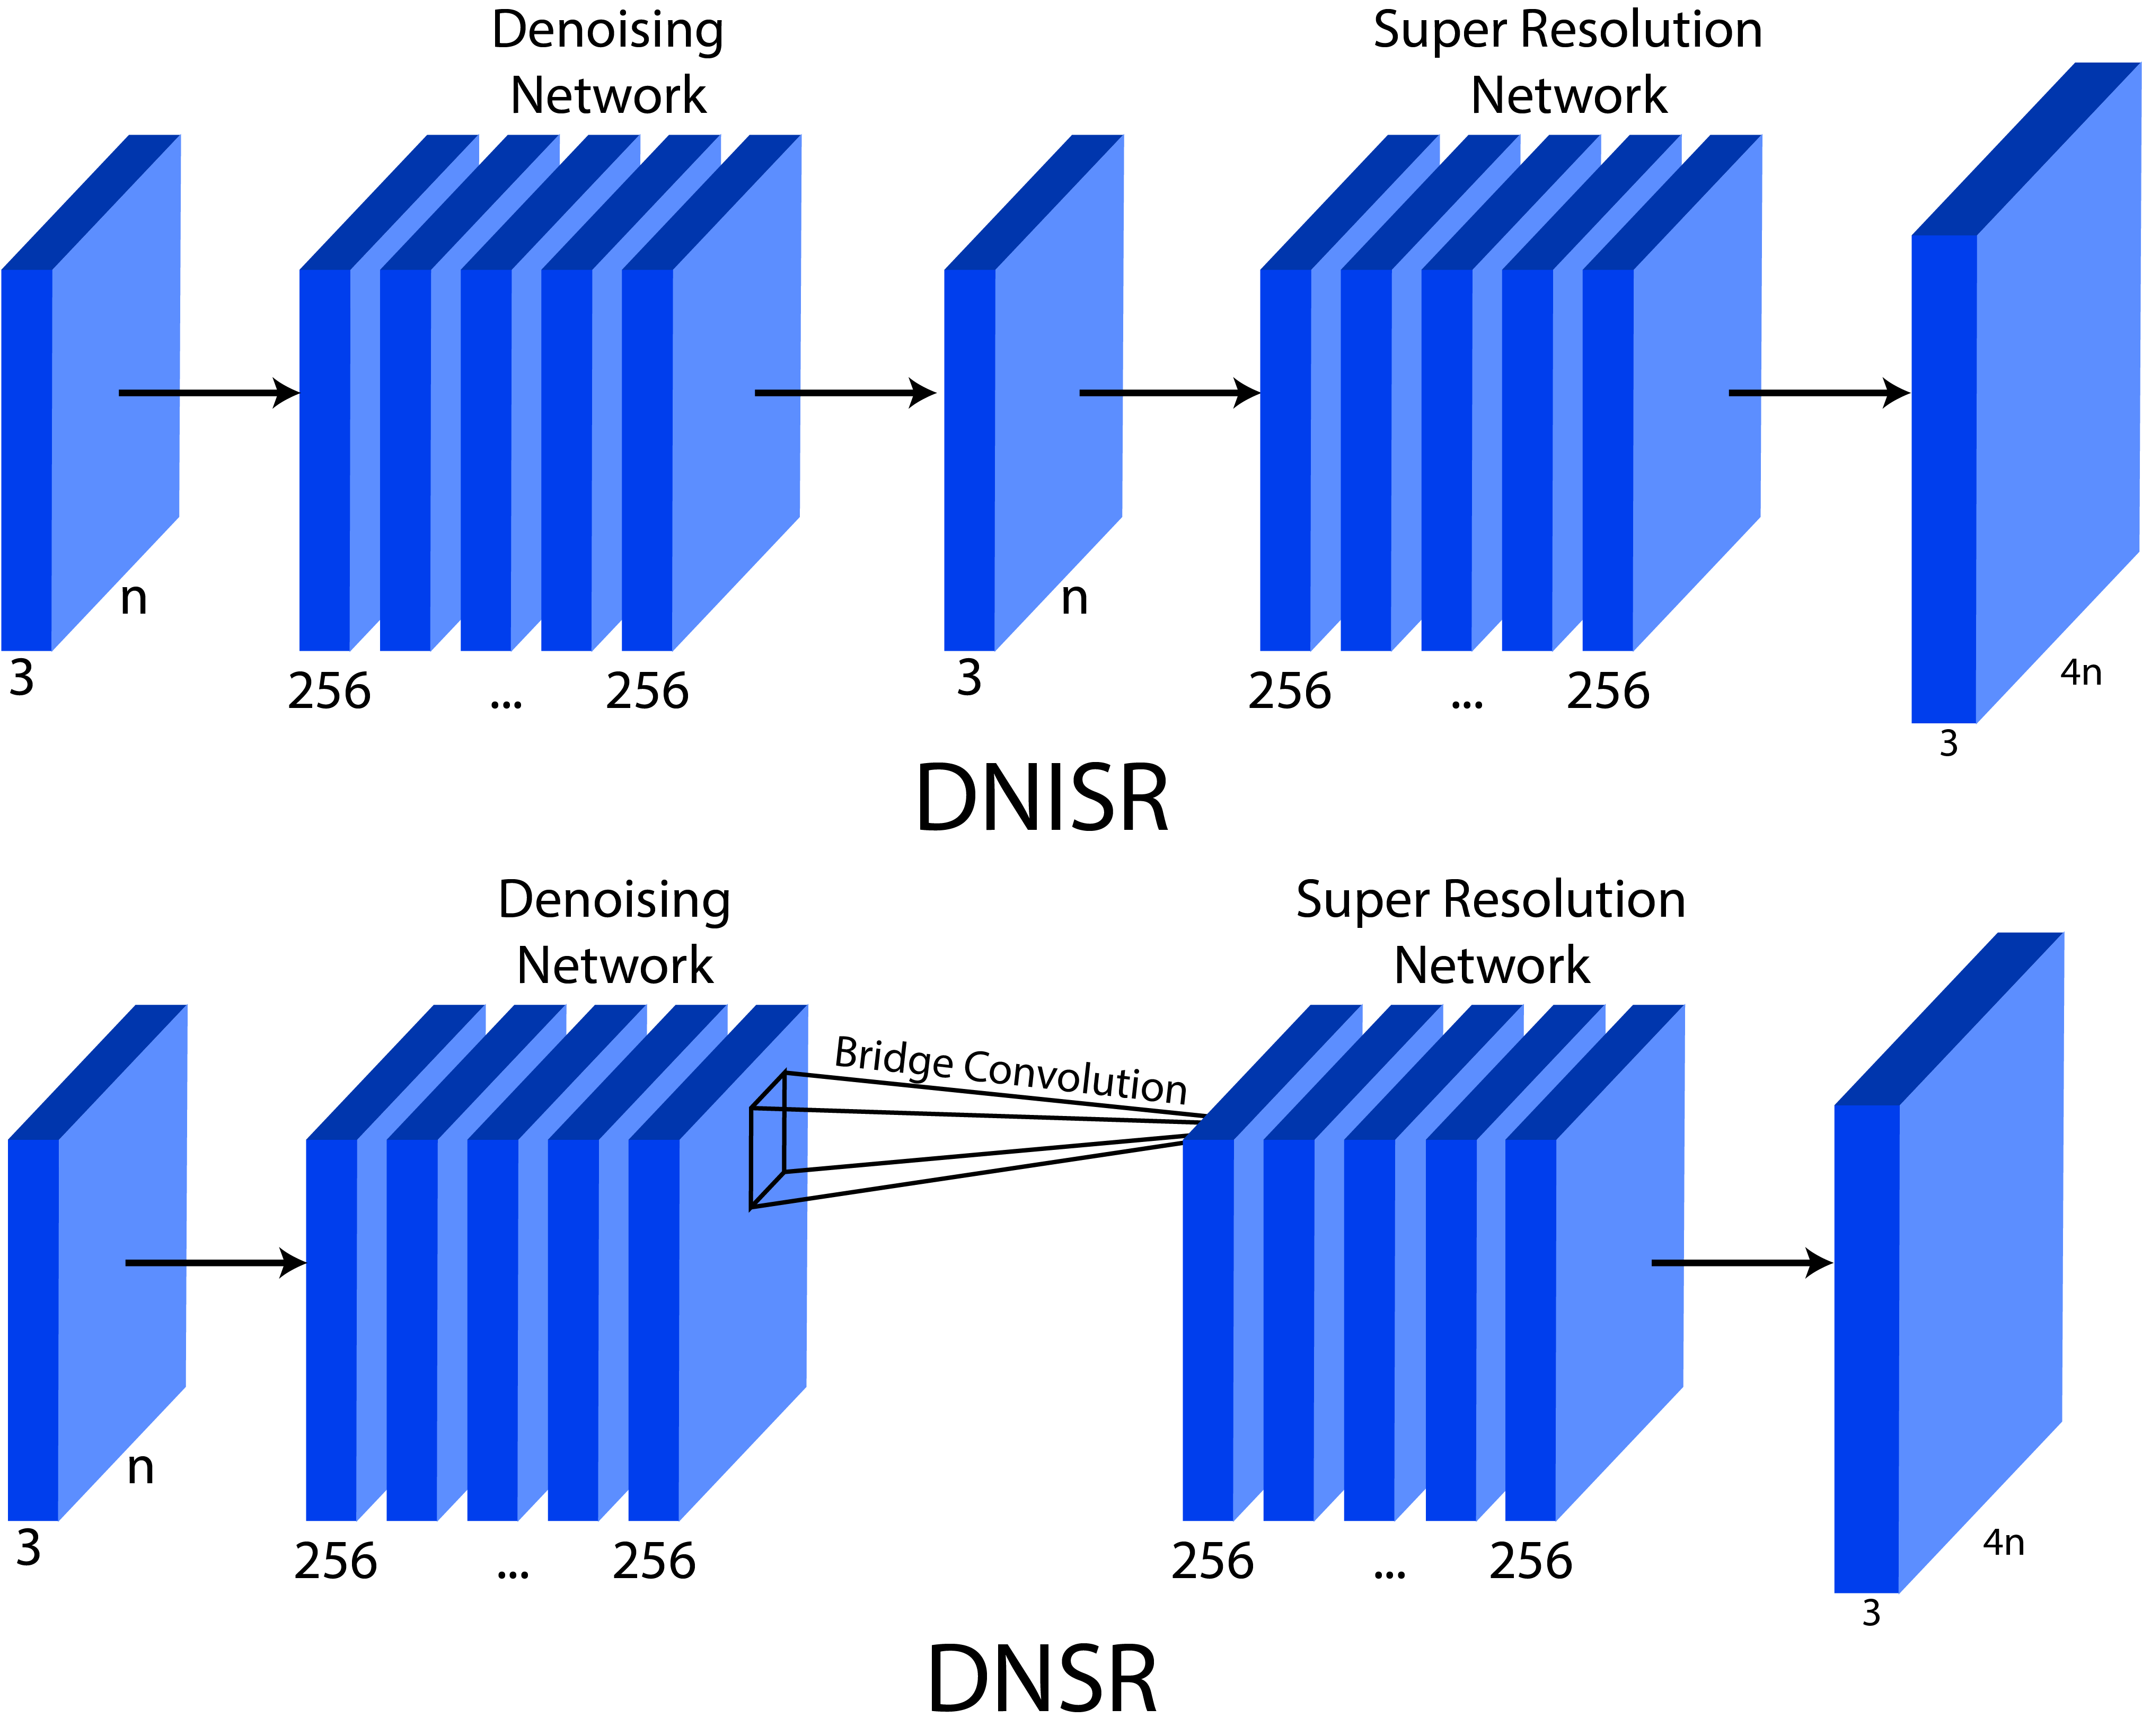
\includegraphics[width=\columnwidth]{Images/DNSR.png}\\
\caption{Architectures for DNSR and DNISR.}
\label{fig:dnsr}
\end{figure}

Table \ref{tbl:dnsr} and Figures \ref{fig:track2diff2} and \ref{fig:track2diff} show a PSNR comparison for EDSR, DNISR, and DNSR. For a visual comparison of the images produced by each algorithm, see Figure \ref{fig:samples}.
\begin{table}[htbp]
    \centering
    \begin{tabular}{c|c|c|c|c}
       Algorithm & BICUBIC & EDSR & DNISR & DNSR \\\hline
       PNSR & 23.47 & 24.49 & 24.52 & \textcolor{red}{24.90} \\
       SSIM & 0.7333 & 0.7925 & 0.7940& \textcolor{red}{0.7956}
    \end{tabular}
    \caption{Comparison of results from EDSR and our denoising networks. The numbers reported were computed on the DIV2K \cite{Agustsson_2017_CVPR_Workshops} validation data set.}
    \label{tbl:dnsr}
\end{table}

\begin{figure}[htbp]
\centering
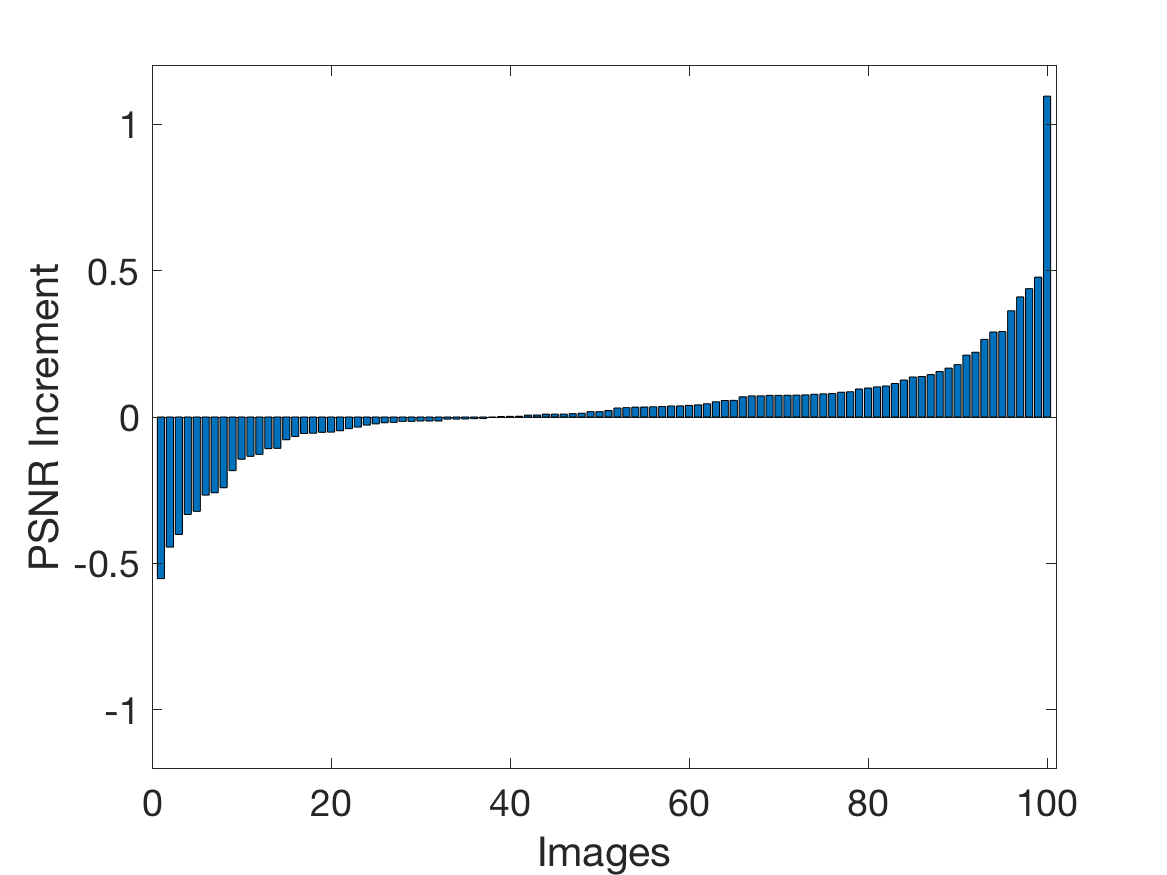
\includegraphics[width=\columnwidth]{Images/Track2DIFF2.png}\\
\caption{PSNR difference between DNISR and EDSR (sorted by difference in PSNR) on the 100 image validation set from DIV2K \cite{Agustsson_2017_CVPR_Workshops}.}
\label{fig:track2diff2}
\end{figure}

\begin{figure}[htbp]
\centering
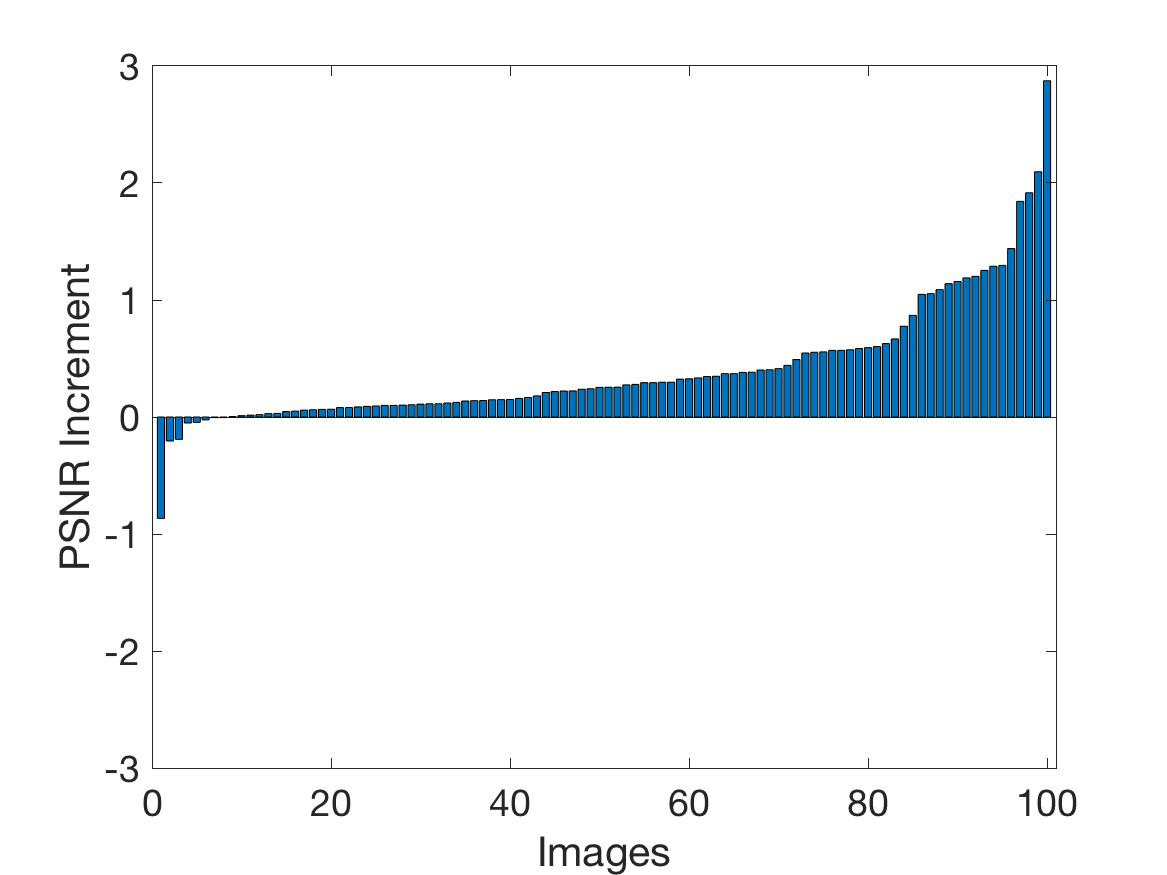
\includegraphics[width=\columnwidth]{Images/Track2DIFF.png}\\
\caption{PSNR difference between DNSR and EDSR (sorted by difference in PSNR) on the 100 image validation set from DIV2K \cite{Agustsson_2017_CVPR_Workshops}}
\label{fig:track2diff}
\end{figure}

%\section{Implementation Details}
%Both augmented training and test time augmentation improved the quality of the model. For Track 1, getting additional external data also improved the model's ability to generalize. This was not possible for Track 2, due to our inability to perfectly replicate the degradations applied to each image. While training the models, we used Cosine Annealing with Warm Restarts to get faster convergence time than in the original EDSR paper. (See Figure ???).

\section{General Tricks and Insights}
We discovered several tricks that can be used any time, with almost any network architecture. To see the results these tricks had on upscaling images by a factor of $8$, see Figure \ref{fig:samples}.
\begin{itemize}
	\item RGB Layer Shuffle: In addition to flipping and rotating the image patches during training and generation, we randomly shuffled the red, green, and blue layers. This improved our overall model by a small amount. This trick is applicable to any convolutional structure. Figure \ref{fig:rgbshuffling} shows the effect of test-time RGB Shuffling.
	\item Per-Image Mean Shift: Instead of calculating the average mean throughout all of the images and normalizing by that value, as in the original EDSR paper, we instead normalized each individual image patch during training by subtracting its mean.
	\item Different Upsampling Techniques: For Track 1, we started by using sub-pixel shift to upscale the image. In addition, to upsample by a factor of $8$, we concatenated three $\times 2$ upsamplers, as in the original EDSR paper. Using this approach, we ran into artifacts induced by the upscaling (see Figure \ref{fig:artifacts}). These artifacts were diminished by switching the upsampling method to Transposed Convolution upsampling. However, even with the sub-pixel shift upscaler, the problem went away when we switched to directly learning a $\times 8$ upscaler instead of three concatenated $\times 2$ upscalers.
	
	In our final method, we found that direct $\times 8$ upscaling combined with the sub-pixel shift upscaler produced images with higher PSNR values. However, the concatenated $\times 2$ upscalers seemed less prone to creating artifacts due to antialiasing (see Figure \ref{fig:antialias}).
	
	\begin{figure}[htbp]
	    \centering
	    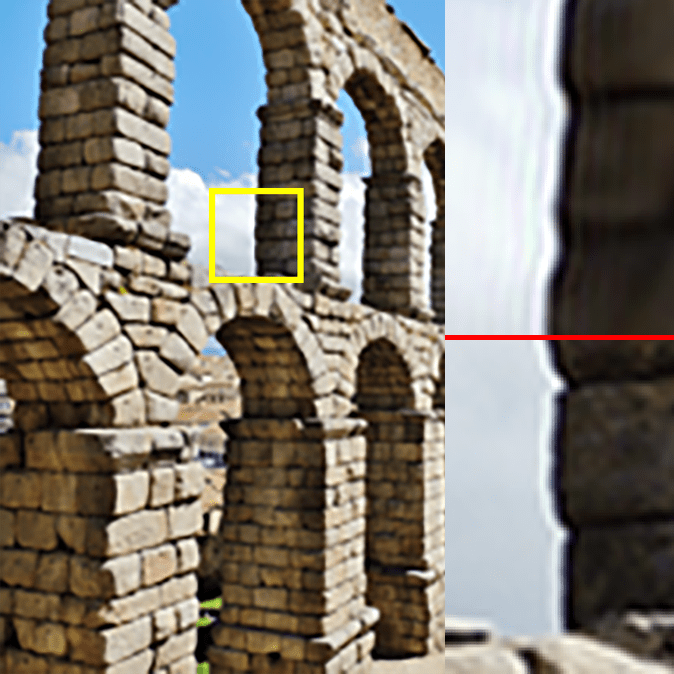
\includegraphics[width=\columnwidth]{Images/artifacts.png}
	    \caption{The upscaler using sub-pixel shift (top-right) has clear chromatic artifacts, while the upscaler using transposed convolutional upscaling (bottom-right) does not.}
	    \label{fig:artifacts}
	\end{figure}
	
	\begin{figure}[htbp]
	    \centering
	    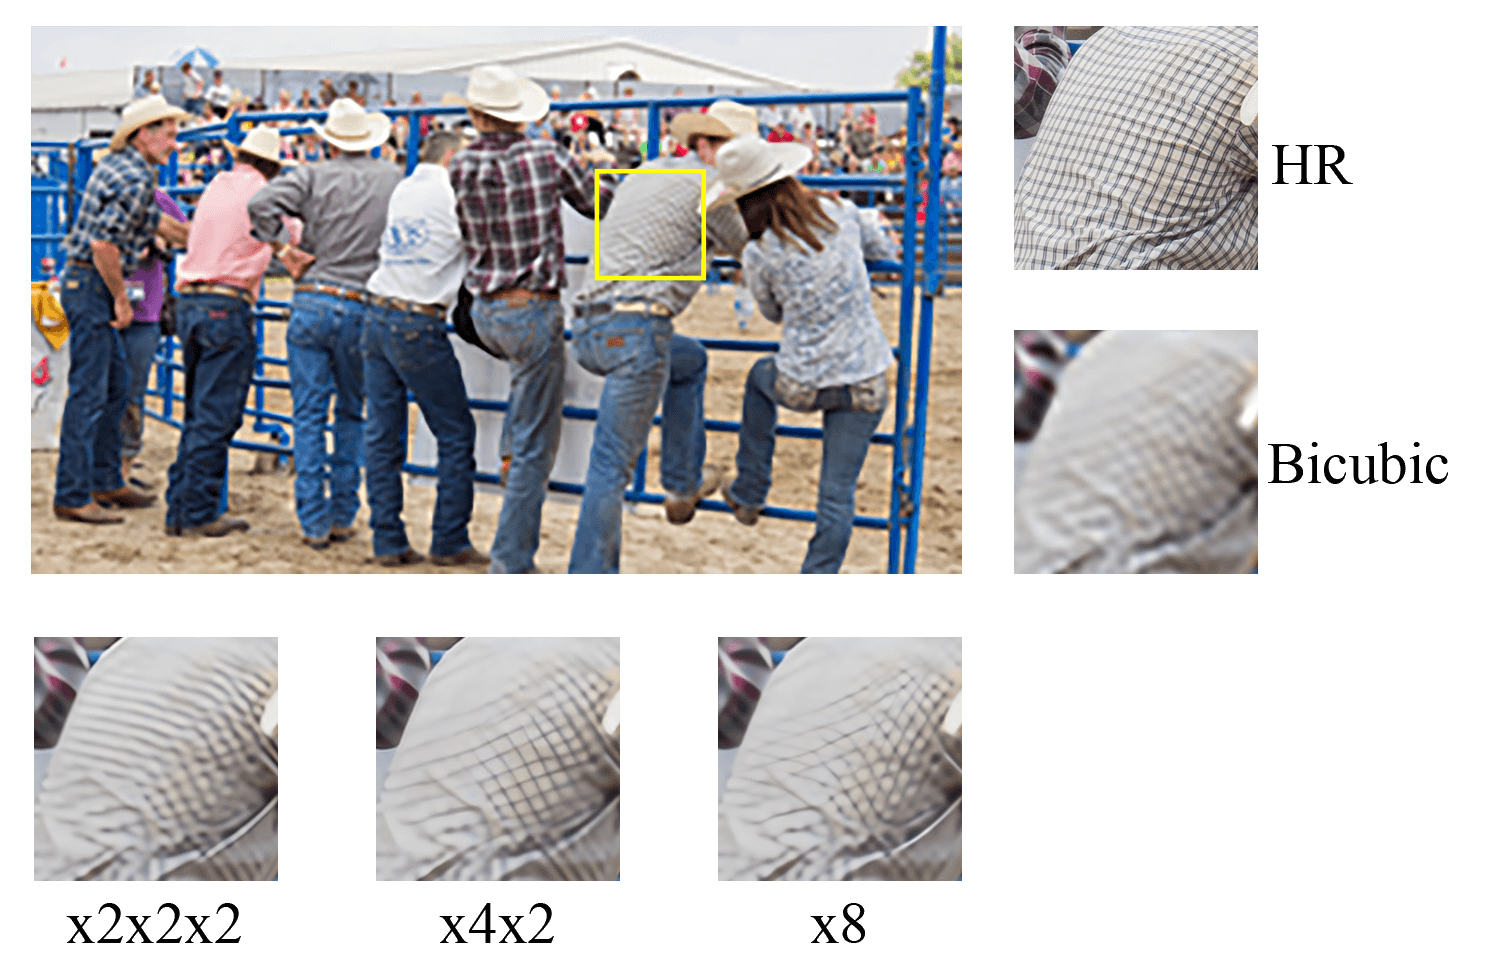
\includegraphics[width=\columnwidth]{Images/Stripes.png}
	    \caption{Diagonal lines created by some upscaling methods due to anti-aliasing}
	    \label{fig:antialias}
	\end{figure}
	
	\item Residual Scaling Factor: In EDSR, each residual layer is multiplied by $0.1$ at the end. Instead of hardcoding this parameter, we allowed it to be a free variable that could be trained.
	\item Edge Loss: We attempted to add an edge-loss component to the loss by applying a Sobel filter to both the upscaled and ground-truth images, and comparing those. However, this did not improve on our previous model.
	\item Kernel Size: We tried various kernel sizes, however $2\times2$ produced worse results and we could not successfully train the network with the $4\times4$ and $5\times5$ kernel sizes.
\end{itemize}

Figure \ref{fig:convergence} shows a comparison of convergence rates for baseline EDSR, EDSR with per image intensity shift, and EDSR with dynamic residual scaling factors. All training started with randomly initialized weights. Using per-image mean shift gives a higher initial PSNR and faster convergence.

\begin{figure}
    \centering
    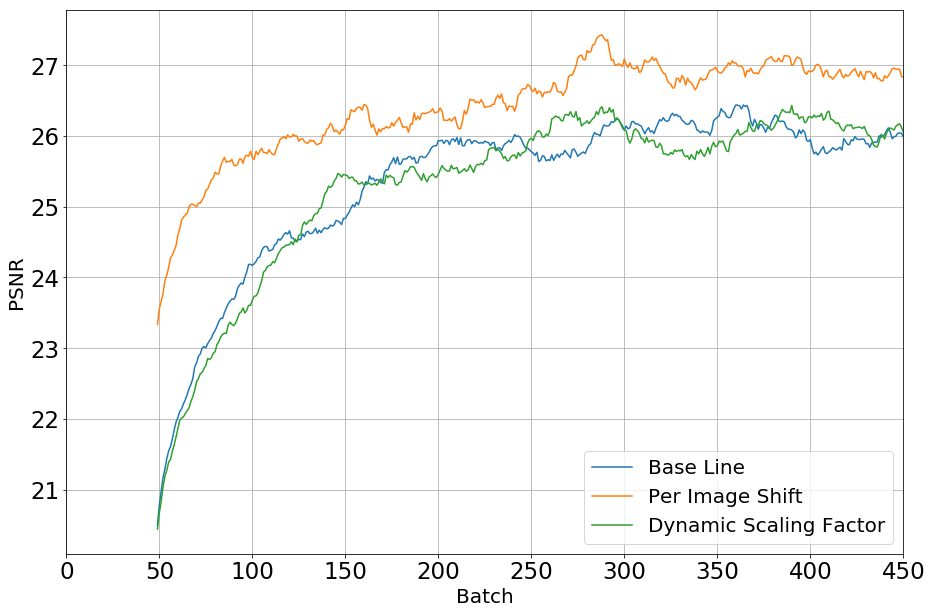
\includegraphics[width=\columnwidth]{Images/convergence.png}
    \caption{Convergence rates for baseline EDSR, EDSR with per image shift and dynamic scaling factor. The figure is plotted with rolling mean of 50.}
    \label{fig:convergence}
\end{figure}

Table \ref{tbl:tricks} and Figure \ref{fig:track1diff} show a PSNR comparison for VDSR, EDSR, and our improved EDSR model. For a visual comparison of the images produced by each algorithm, see Figure \ref{fig:samples}.

\begin{table}[ht!]
    \centering
    \begin{tabular}{c|c|c|c|c}
       \footnotesize{Algorithm}  & \footnotesize{EDSR} & \footnotesize{Improved} \footnotesize{EDSR} & \footnotesize{VDSR} & \footnotesize{BICUBIC}\\ \hline
        \footnotesize{PNSR} & 25.49 & \textcolor{red}{25.60} & 24.70 & 23.69 \\
        \footnotesize{SSIM} & 0.6930 & \textcolor{red}{0.6974} & 0.6580 & 0.6291\\
    \end{tabular}
    \caption{Comparison of our improved EDSR algorithm to several baselines. The improvements could have been made to any SR algorithm besides EDSR. The numbers reported were computed on the DIV2K validation data set.}
    \label{tbl:tricks}
\end{table}

\begin{figure}[htbp]
\centering
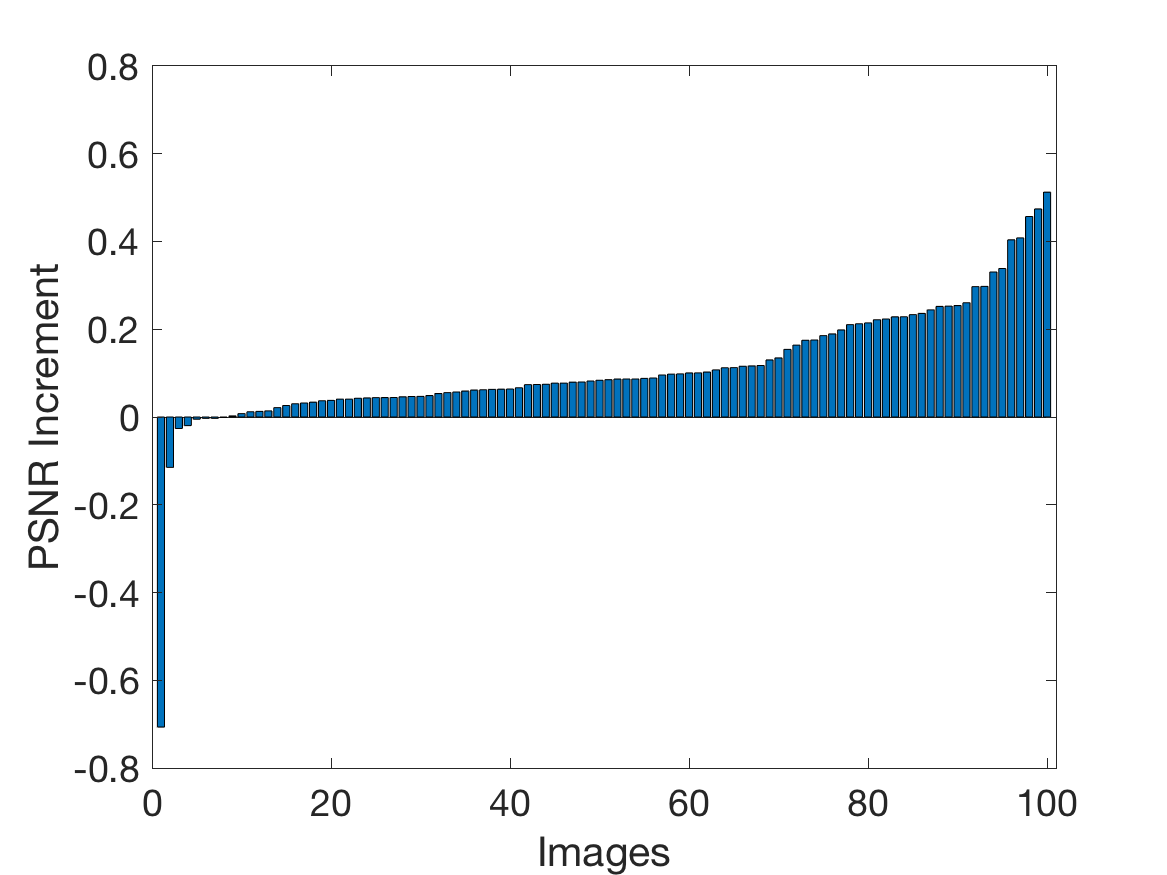
\includegraphics[width=\columnwidth]{Images/Track1DIFF.png}\\
\caption{PSNR difference between our improved EDSR and baseline EDSR (sorted by difference in PSNR) on the 100 image validation set from DIV2K \cite{Agustsson_2017_CVPR_Workshops}.}
\label{fig:track1diff}
\end{figure}

\begin{figure}[ht]
    \centering
    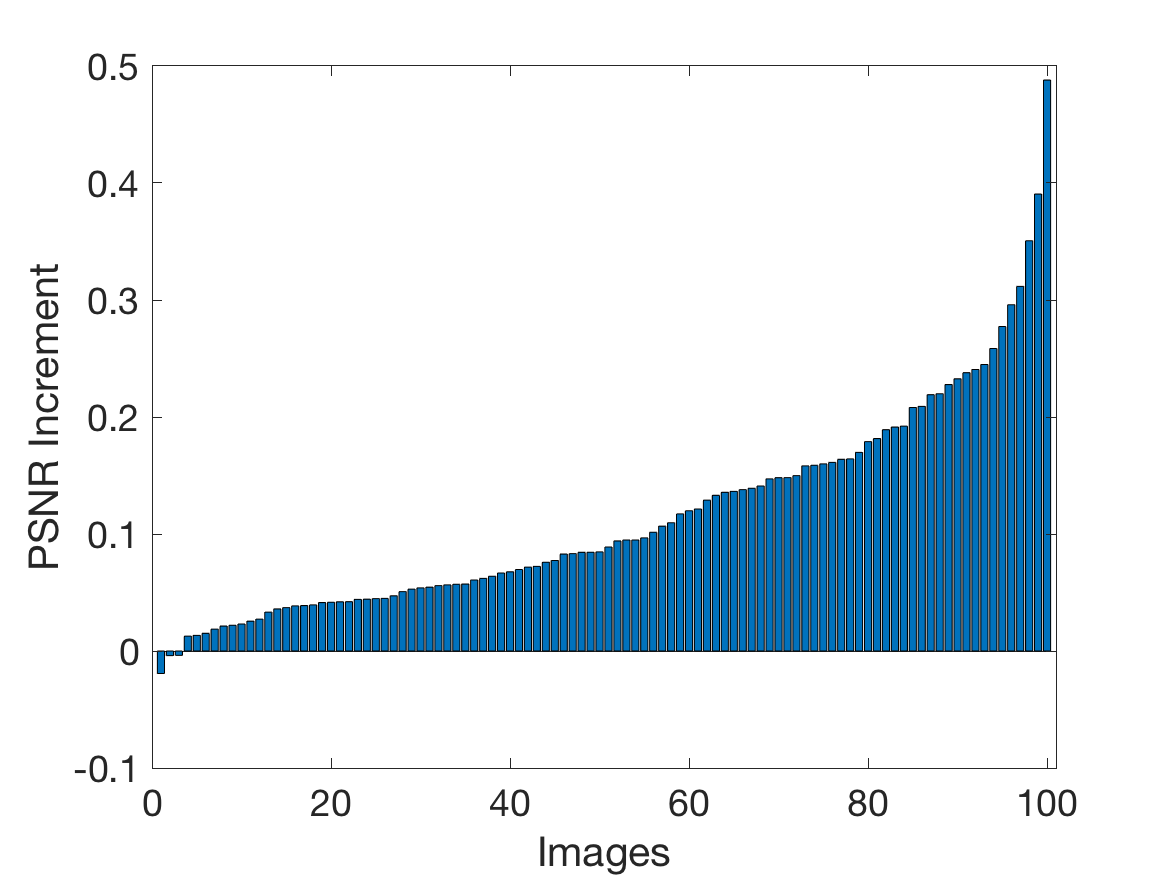
\includegraphics[width=\columnwidth]{Images/RGBShuffling.png}
    \caption{PSNR increment from test time RGB Shuffling (sorted by difference in PSNR)}
    \label{fig:rgbshuffling}
\end{figure}

Figure \ref{fig:rgbshuffling} shows the PSNR increment across the 100 images from the DIV2K validation set after applying only RGB Shuffling to EDSR. In 97 out of the 100 cases, there was a boost in PSNR.
\section{Conclusion}
We discussed two new network architectures for denoising and preserving general structure in images during super-resolution, as well as a toolbox of tricks. The vast majority of the findings described here were not implemented in time for the competition deadline. Our high-scoring entries are mostly a result of the toolbox of tricks discussed above. 
We have noticed substantial improvement from our competition entries to the results reported in this paper.

Our code is available at: \url{https://github.com/websterbei/EDSR_tensorflow} and \url{https://github.com/nikhilvravi/DukeSR}.

\begin{figure*}[ht!]
\centering
\begin{subfigure}[t]{0.4\textwidth}
    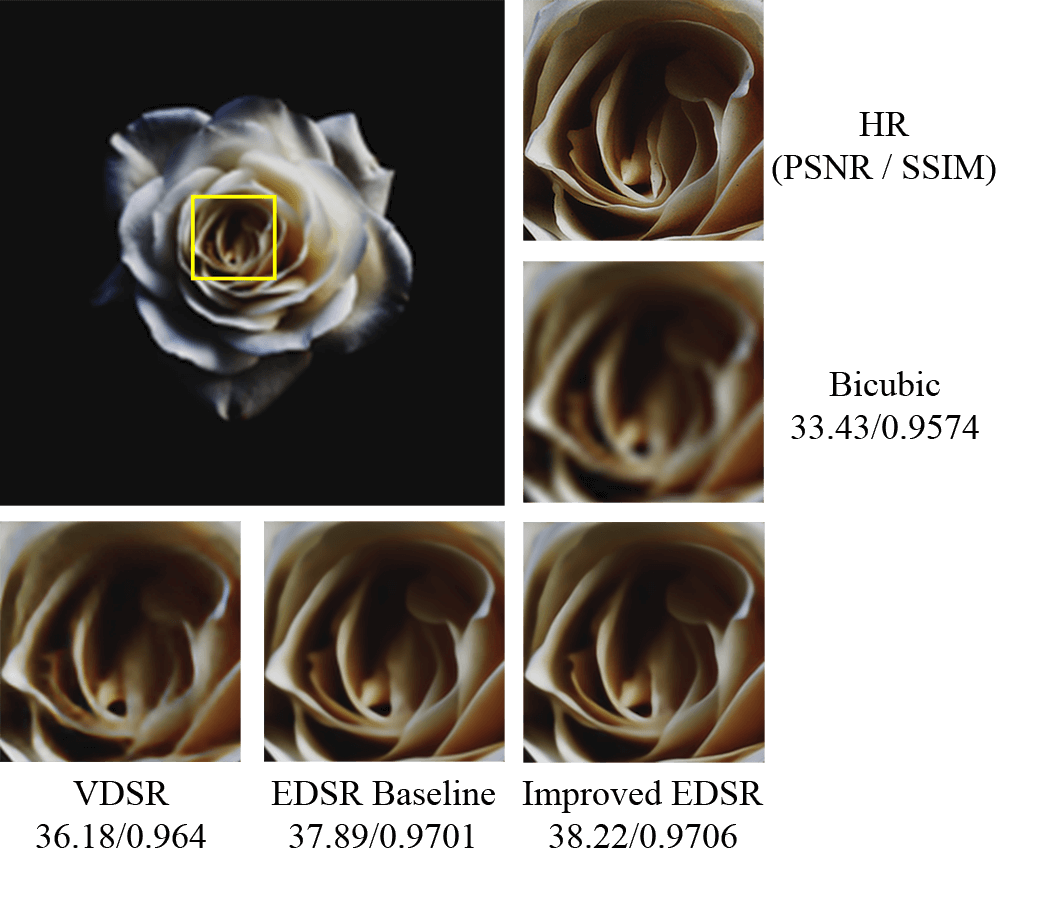
\includegraphics[width=\textwidth]{Images/Samples/1-2.png}\\
    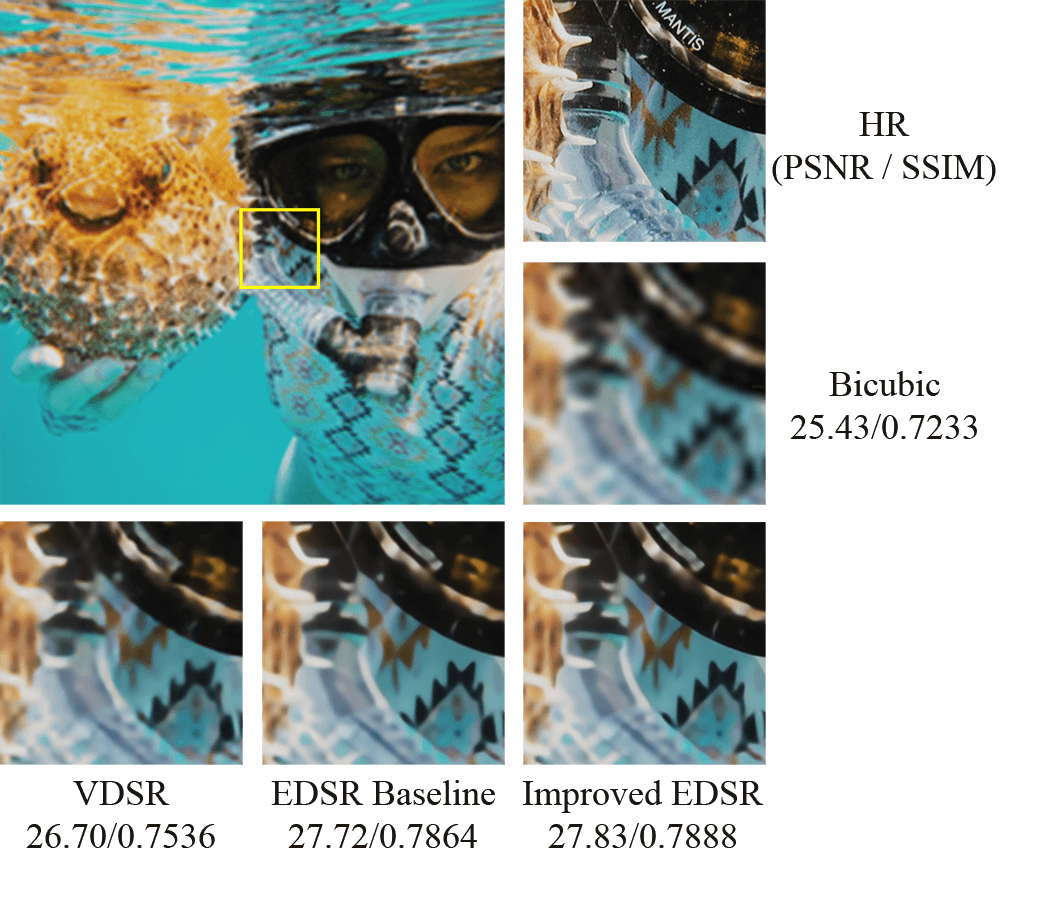
\includegraphics[width=\textwidth]{Images/Samples/1-1.png}\\
    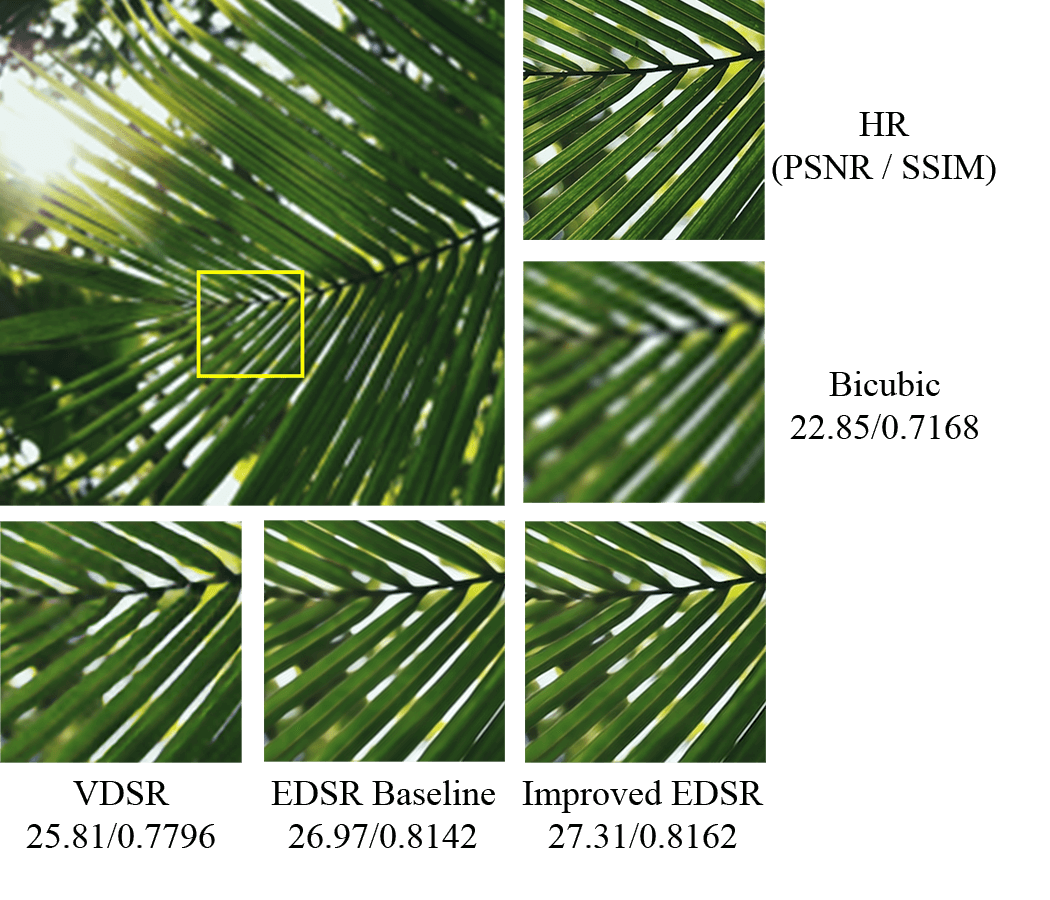
\includegraphics[width=\textwidth]{Images/Samples/1-3.png}
\end{subfigure}
\hspace{0.05\textwidth}
\vrule
\hspace{0.1\textwidth}
\begin{subfigure}[t]{0.4\textwidth}
    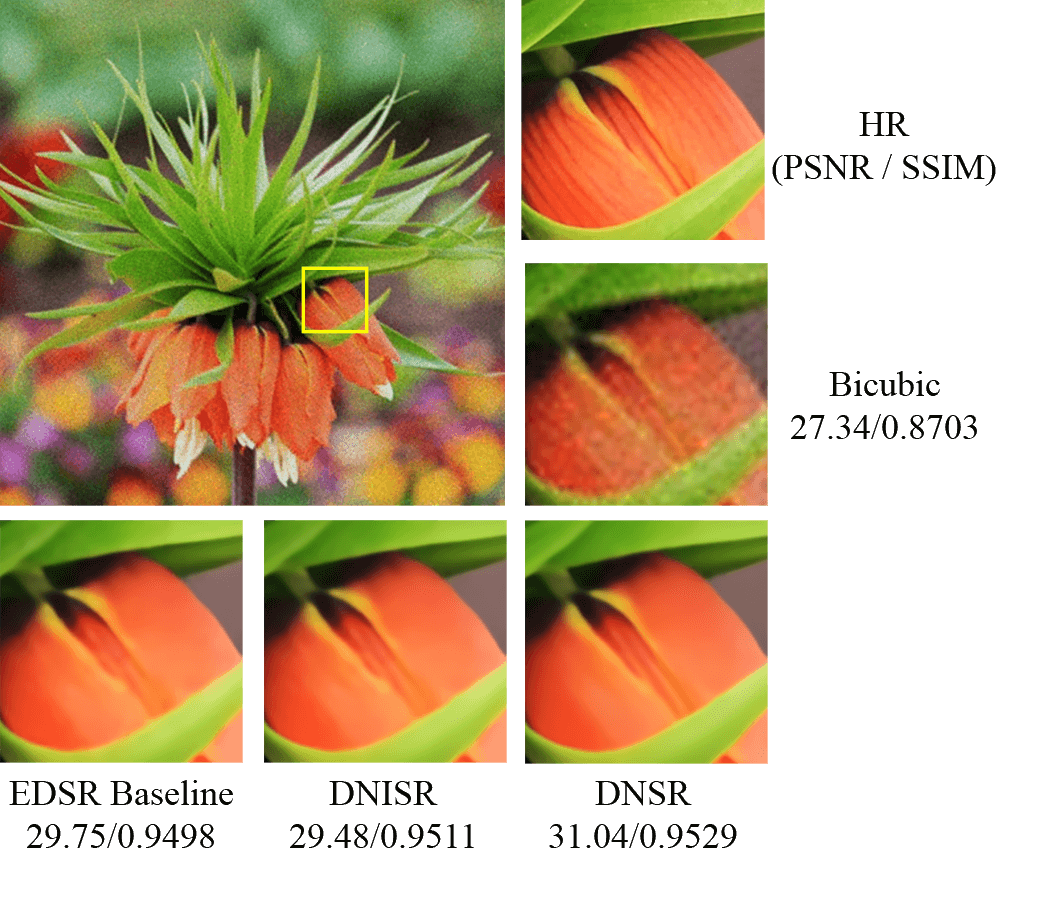
\includegraphics[width=\textwidth]{Images/Samples/2-1.png}\\
    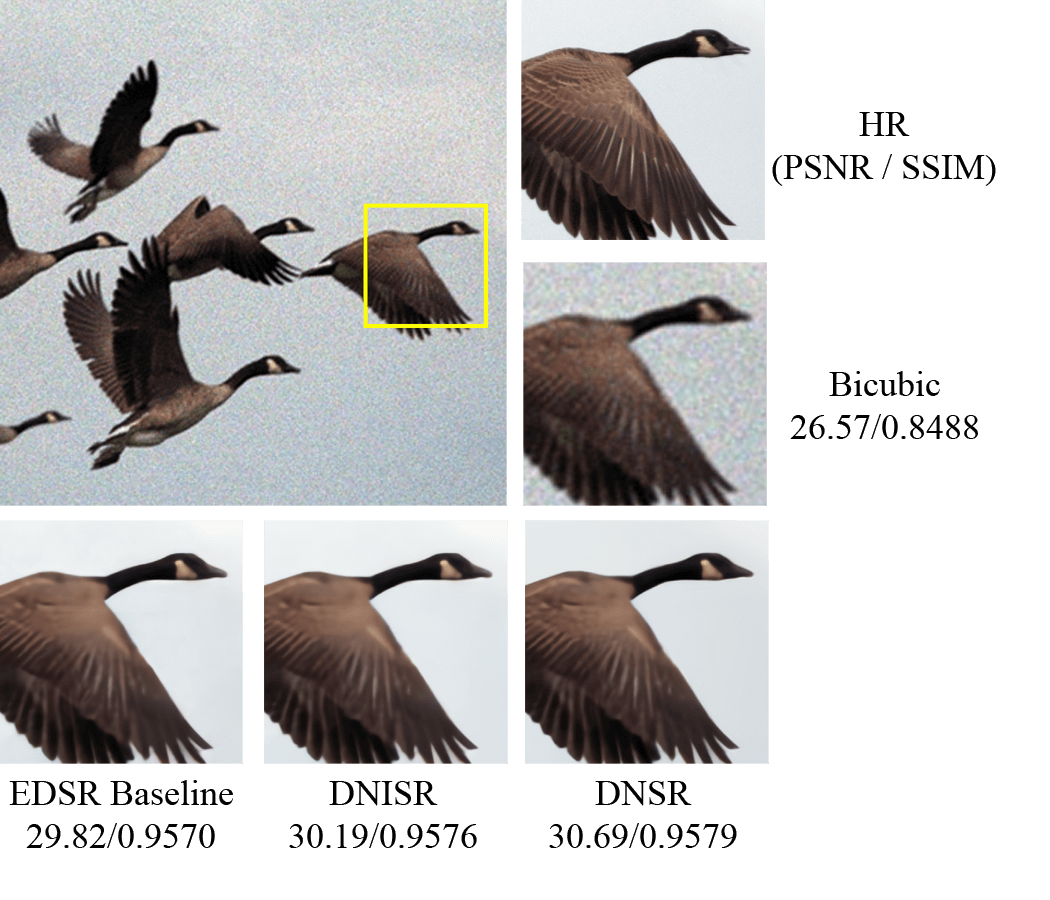
\includegraphics[width=\textwidth]{Images/Samples/2-2.png}\\
    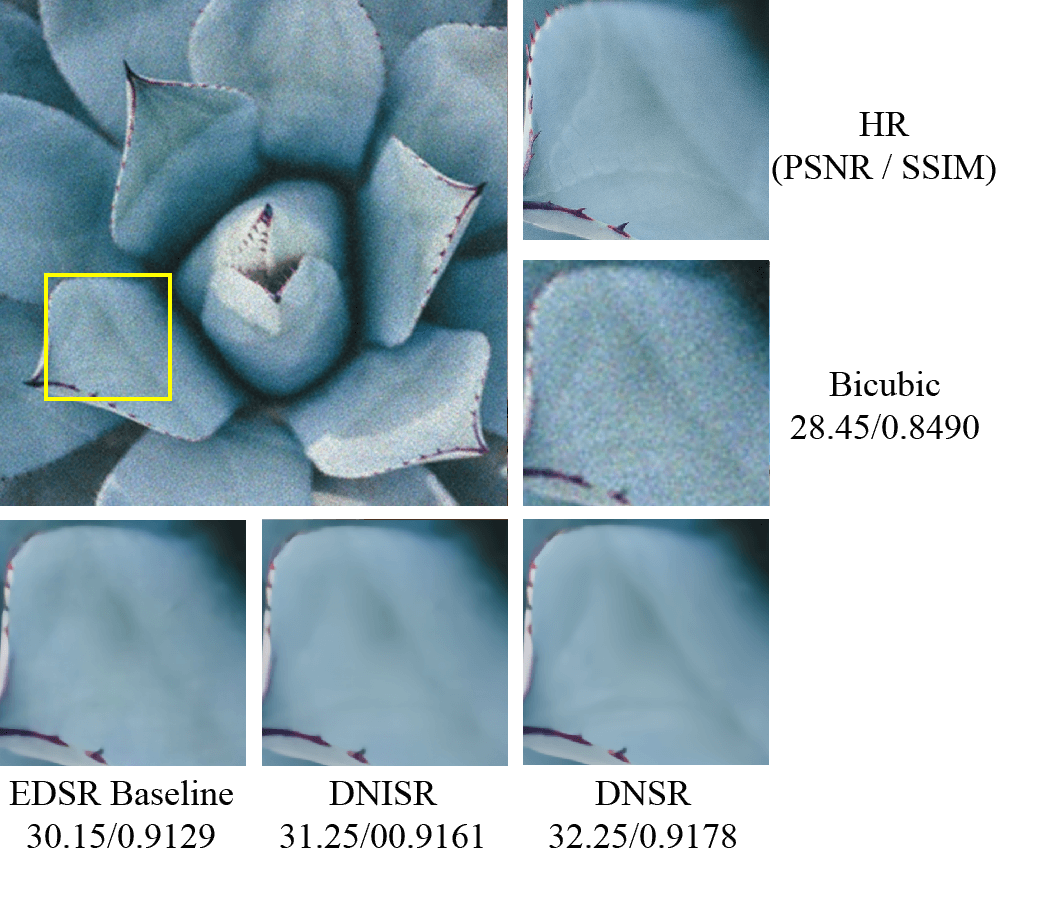
\includegraphics[width=\textwidth]{Images/Samples/2-3.png}
\end{subfigure}
\caption{Comparison of different techniques for upscaling images by a factor of 8 (left) and upscaling noisy images by a factor of 4 (right). The visual differences between the images are especially pronounced in the last images of each column, where the folds in the leaves are much clearer.}
\label{fig:samples}
\end{figure*}

{\small
\bibliographystyle{ieee}
\bibliography{egbib}
}

\end{document}

\documentclass[10pt,twocolumn,letterpaper]{article}

\usepackage{cvpr}
\usepackage{times}
\usepackage{epsfig}
\usepackage{graphicx}
\usepackage{amsmath}
\usepackage{amssymb}

% Include other packages here, before hyperref.

% If you comment hyperref and then uncomment it, you should delete
% egpaper.aux before re-running latex.  (Or just hit 'q' on the first latex
% run, let it finish, and you should be clear).
\usepackage[pagebackref=true,breaklinks=true,letterpaper=true,colorlinks,bookmarks=false]{hyperref}

% \cvprfinalcopy % *** Uncomment this line for the final submission

\def\cvprPaperID{****} % *** Enter the CVPR Paper ID here
\def\httilde{\mbox{\tt\raisebox{-.5ex}{\symbol{126}}}}

% Pages are numbered in submission mode, and unnumbered in camera-ready
\ifcvprfinal\pagestyle{empty}\fi
\begin{document}

%%%%%%%%% TITLE
\title{\LaTeX\ Author Guidelines for CVPR Proceedings}

\author{First Author\\
Institution1\\
Institution1 address\\
{\tt\small firstauthor@i1.org}
% For a paper whose authors are all at the same institution,
% omit the following lines up until the closing ``}''.
% Additional authors and addresses can be added with ``\and'',
% just like the second author.
% To save space, use either the email address or home page, not both
\and
Second Author\\
Institution2\\
First line of institution2 address\\
{\tt\small secondauthor@i2.org}
}

\maketitle
%\thispagestyle{empty}

%%%%%%%%% ABSTRACT
\begin{abstract}
   The ABSTRACT is to be in fully-justified italicized text, at the top
   of the left-hand column, below the author and affiliation
   information. Use the word ``Abstract'' as the title, in 12-point
   Times, boldface type, centered relative to the column, initially
   capitalized. The abstract is to be in 10-point, single-spaced type.
   Leave two blank lines after the Abstract, then begin the main text.
   Look at previous CVPR abstracts to get a feel for style and length.
\end{abstract}

%%%%%%%%% BODY TEXT
\section{Introduction}

Please follow the steps outlined below when submitting your manuscript to
the IEEE Computer Society Press.  This style guide now has several
important modifications (for example, you are no longer warned against the
use of sticky tape to attach your artwork to the paper), so all authors
should read this new version.

%-------------------------------------------------------------------------
\subsection{Language}

All manuscripts must be in English.

\subsection{Dual submission}

Please refer to the author guidelines on the CVPR 2018 web page for a
discussion of the policy on dual submissions.

\subsection{Paper length}
Papers, excluding the references section,
must be no longer than eight pages in length. The references section
will not be included in the page count, and there is no limit on the
length of the references section. For example, a paper of eight pages
with two pages of references would have a total length of 10 pages.
{\bf There will be no extra page charges for CVPR 2018.}

Overlength papers will simply not be reviewed.  This includes papers
where the margins and formatting are deemed to have been significantly
altered from those laid down by this style guide.  Note that this
\LaTeX\ guide already sets figure captions and references in a smaller font.
The reason such papers will not be reviewed is that there is no provision for
supervised revisions of manuscripts.  The reviewing process cannot determine
the suitability of the paper for presentation in eight pages if it is
reviewed in eleven.  

%-------------------------------------------------------------------------
\subsection{The ruler}
The \LaTeX\ style defines a printed ruler which should be present in the
version submitted for review.  The ruler is provided in order that
reviewers may comment on particular lines in the paper without
circumlocution.  If you are preparing a document using a non-\LaTeX\
document preparation system, please arrange for an equivalent ruler to
appear on the final output pages.  The presence or absence of the ruler
should not change the appearance of any other content on the page.  The
camera ready copy should not contain a ruler. (\LaTeX\ users may uncomment
the \verb'\cvprfinalcopy' command in the document preamble.)  Reviewers:
note that the ruler measurements do not align well with lines in the paper
--- this turns out to be very difficult to do well when the paper contains
many figures and equations, and, when done, looks ugly.  Just use fractional
references (e.g.\ this line is $095.5$), although in most cases one would
expect that the approximate location will be adequate.

\subsection{Mathematics}

Please number all of your sections and displayed equations.  It is
important for readers to be able to refer to any particular equation.  Just
because you didn't refer to it in the text doesn't mean some future reader
might not need to refer to it.  It is cumbersome to have to use
circumlocutions like ``the equation second from the top of page 3 column
1''.  (Note that the ruler will not be present in the final copy, so is not
an alternative to equation numbers).  All authors will benefit from reading
Mermin's description of how to write mathematics:
\url{http://www.pamitc.org/documents/mermin.pdf}.


\subsection{Blind review}

Many authors misunderstand the concept of anonymizing for blind
review.  Blind review does not mean that one must remove
citations to one's own work---in fact it is often impossible to
review a paper unless the previous citations are known and
available.

Blind review means that you do not use the words ``my'' or ``our''
when citing previous work.  That is all.  (But see below for
techreports.)

Saying ``this builds on the work of Lucy Smith [1]'' does not say
that you are Lucy Smith; it says that you are building on her
work.  If you are Smith and Jones, do not say ``as we show in
[7]'', say ``as Smith and Jones show in [7]'' and at the end of the
paper, include reference 7 as you would any other cited work.

An example of a bad paper just asking to be rejected:
\begin{quote}
\begin{center}
    An analysis of the frobnicatable foo filter.
\end{center}

   In this paper we present a performance analysis of our
   previous paper [1], and show it to be inferior to all
   previously known methods.  Why the previous paper was
   accepted without this analysis is beyond me.

   [1] Removed for blind review
\end{quote}


An example of an acceptable paper:

\begin{quote}
\begin{center}
     An analysis of the frobnicatable foo filter.
\end{center}

   In this paper we present a performance analysis of the
   paper of Smith \etal [1], and show it to be inferior to
   all previously known methods.  Why the previous paper
   was accepted without this analysis is beyond me.

   [1] Smith, L and Jones, C. ``The frobnicatable foo
   filter, a fundamental contribution to human knowledge''.
   Nature 381(12), 1-213.
\end{quote}

If you are making a submission to another conference at the same time,
which covers similar or overlapping material, you may need to refer to that
submission in order to explain the differences, just as you would if you
had previously published related work.  In such cases, include the
anonymized parallel submission~\cite{Authors14} as additional material and
cite it as
\begin{quote}
[1] Authors. ``The frobnicatable foo filter'', F\&G 2014 Submission ID 324,
Supplied as additional material {\tt fg324.pdf}.
\end{quote}

Finally, you may feel you need to tell the reader that more details can be
found elsewhere, and refer them to a technical report.  For conference
submissions, the paper must stand on its own, and not {\em require} the
reviewer to go to a techreport for further details.  Thus, you may say in
the body of the paper ``further details may be found
in~\cite{Authors14b}''.  Then submit the techreport as additional material.
Again, you may not assume the reviewers will read this material.

Sometimes your paper is about a problem which you tested using a tool which
is widely known to be restricted to a single institution.  For example,
let's say it's 1969, you have solved a key problem on the Apollo lander,
and you believe that the CVPR70 audience would like to hear about your
solution.  The work is a development of your celebrated 1968 paper entitled
``Zero-g frobnication: How being the only people in the world with access to
the Apollo lander source code makes us a wow at parties'', by Zeus \etal.

You can handle this paper like any other.  Don't write ``We show how to
improve our previous work [Anonymous, 1968].  This time we tested the
algorithm on a lunar lander [name of lander removed for blind review]''.
That would be silly, and would immediately identify the authors. Instead
write the following:
\begin{quotation}
\noindent
   We describe a system for zero-g frobnication.  This
   system is new because it handles the following cases:
   A, B.  Previous systems [Zeus et al. 1968] didn't
   handle case B properly.  Ours handles it by including
   a foo term in the bar integral.

   ...

   The proposed system was integrated with the Apollo
   lunar lander, and went all the way to the moon, don't
   you know.  It displayed the following behaviours
   which show how well we solved cases A and B: ...
\end{quotation}
As you can see, the above text follows standard scientific convention,
reads better than the first version, and does not explicitly name you as
the authors.  A reviewer might think it likely that the new paper was
written by Zeus \etal, but cannot make any decision based on that guess.
He or she would have to be sure that no other authors could have been
contracted to solve problem B.
\medskip

\noindent
FAQ\medskip\\
{\bf Q:} Are acknowledgements OK?\\
{\bf A:} No.  Leave them for the final copy.\medskip\\
{\bf Q:} How do I cite my results reported in open challenges?
{\bf A:} To conform with the double blind review policy, you can report results of other challenge participants together with your results in your paper. For your results, however, you should not identify yourself and should not mention your participation in the challenge. Instead present your results referring to the method proposed in your paper and draw conclusions based on the experimental comparison to other results.\medskip\\

\begin{figure}[t]
\begin{center}
\fbox{\rule{0pt}{2in} \rule{0.9\linewidth}{0pt}}
   %\includegraphics[width=0.8\linewidth]{egfigure.eps}
\end{center}
   \caption{Example of caption.  It is set in Roman so that mathematics
   (always set in Roman: $B \sin A = A \sin B$) may be included without an
   ugly clash.}
\label{fig:long}
\label{fig:onecol}
\end{figure}

\subsection{Miscellaneous}

\noindent
Compare the following:\\
\begin{tabular}{ll}
 \verb'$conf_a$' &  $conf_a$ \\
 \verb'$\mathit{conf}_a$' & $\mathit{conf}_a$
\end{tabular}\\
See The \TeX book, p165.

The space after \eg, meaning ``for example'', should not be a
sentence-ending space. So \eg is correct, {\em e.g.} is not.  The provided
\verb'\eg' macro takes care of this.

When citing a multi-author paper, you may save space by using ``et alia'',
shortened to ``\etal'' (not ``{\em et.\ al.}'' as ``{\em et}'' is a complete word.)
However, use it only when there are three or more authors.  Thus, the
following is correct: ``
   Frobnication has been trendy lately.
   It was introduced by Alpher~\cite{Alpher02}, and subsequently developed by
   Alpher and Fotheringham-Smythe~\cite{Alpher03}, and Alpher \etal~\cite{Alpher04}.''

This is incorrect: ``... subsequently developed by Alpher \etal~\cite{Alpher03} ...''
because reference~\cite{Alpher03} has just two authors.  If you use the
\verb'\etal' macro provided, then you need not worry about double periods
when used at the end of a sentence as in Alpher \etal.

For this citation style, keep multiple citations in numerical (not
chronological) order, so prefer \cite{Alpher03,Alpher02,Authors14} to
\cite{Alpher02,Alpher03,Authors14}.


\begin{figure*}
\begin{center}
\fbox{\rule{0pt}{2in} \rule{.9\linewidth}{0pt}}
\end{center}
   \caption{Example of a short caption, which should be centered.}
\label{fig:short}
\end{figure*}

%------------------------------------------------------------------------
\section{Formatting your paper}

All text must be in a two-column format. The total allowable width of the
text area is $6\frac78$ inches (17.5 cm) wide by $8\frac78$ inches (22.54
cm) high. Columns are to be $3\frac14$ inches (8.25 cm) wide, with a
$\frac{5}{16}$ inch (0.8 cm) space between them. The main title (on the
first page) should begin 1.0 inch (2.54 cm) from the top edge of the
page. The second and following pages should begin 1.0 inch (2.54 cm) from
the top edge. On all pages, the bottom margin should be 1-1/8 inches (2.86
cm) from the bottom edge of the page for $8.5 \times 11$-inch paper; for A4
paper, approximately 1-5/8 inches (4.13 cm) from the bottom edge of the
page.

%-------------------------------------------------------------------------
\subsection{Margins and page numbering}

All printed material, including text, illustrations, and charts, must be kept
within a print area 6-7/8 inches (17.5 cm) wide by 8-7/8 inches (22.54 cm)
high.



%-------------------------------------------------------------------------
\subsection{Type-style and fonts}

Wherever Times is specified, Times Roman may also be used. If neither is
available on your word processor, please use the font closest in
appearance to Times to which you have access.

MAIN TITLE. Center the title 1-3/8 inches (3.49 cm) from the top edge of
the first page. The title should be in Times 14-point, boldface type.
Capitalize the first letter of nouns, pronouns, verbs, adjectives, and
adverbs; do not capitalize articles, coordinate conjunctions, or
prepositions (unless the title begins with such a word). Leave two blank
lines after the title.

AUTHOR NAME(s) and AFFILIATION(s) are to be centered beneath the title
and printed in Times 12-point, non-boldface type. This information is to
be followed by two blank lines.

The ABSTRACT and MAIN TEXT are to be in a two-column format.

MAIN TEXT. Type main text in 10-point Times, single-spaced. Do NOT use
double-spacing. All paragraphs should be indented 1 pica (approx. 1/6
inch or 0.422 cm). Make sure your text is fully justified---that is,
flush left and flush right. Please do not place any additional blank
lines between paragraphs.

Figure and table captions should be 9-point Roman type as in
Figures~\ref{fig:onecol} and~\ref{fig:short}.  Short captions should be centred.

\noindent Callouts should be 9-point Helvetica, non-boldface type.
Initially capitalize only the first word of section titles and first-,
second-, and third-order headings.

FIRST-ORDER HEADINGS. (For example, {\large \bf 1. Introduction})
should be Times 12-point boldface, initially capitalized, flush left,
with one blank line before, and one blank line after.

SECOND-ORDER HEADINGS. (For example, { \bf 1.1. Database elements})
should be Times 11-point boldface, initially capitalized, flush left,
with one blank line before, and one after. If you require a third-order
heading (we discourage it), use 10-point Times, boldface, initially
capitalized, flush left, preceded by one blank line, followed by a period
and your text on the same line.

%-------------------------------------------------------------------------
\subsection{Footnotes}

Please use footnotes\footnote {This is what a footnote looks like.  It
often distracts the reader from the main flow of the argument.} sparingly.
Indeed, try to avoid footnotes altogether and include necessary peripheral
observations in
the text (within parentheses, if you prefer, as in this sentence).  If you
wish to use a footnote, place it at the bottom of the column on the page on
which it is referenced. Use Times 8-point type, single-spaced.


%-------------------------------------------------------------------------
\subsection{References}

List and number all bibliographical references in 9-point Times,
single-spaced, at the end of your paper. When referenced in the text,
enclose the citation number in square brackets, for
example~\cite{Authors14}.  Where appropriate, include the name(s) of
editors of referenced books.

\begin{table}
\begin{center}
\begin{tabular}{|l|c|}
\hline
Method & Frobnability \\
\hline\hline
Theirs & Frumpy \\
Yours & Frobbly \\
Ours & Makes one's heart Frob\\
\hline
\end{tabular}
\end{center}
\caption{Results.   Ours is better.}
\end{table}

%-------------------------------------------------------------------------
\subsection{Illustrations, graphs, and photographs}

All graphics should be centered.  Please ensure that any point you wish to
make is resolvable in a printed copy of the paper.  Resize fonts in figures
to match the font in the body text, and choose line widths which render
effectively in print.  Many readers (and reviewers), even of an electronic
copy, will choose to print your paper in order to read it.  You cannot
insist that they do otherwise, and therefore must not assume that they can
zoom in to see tiny details on a graphic.

When placing figures in \LaTeX, it's almost always best to use
\verb+\includegraphics+, and to specify the  figure width as a multiple of
the line width as in the example below
{\small\begin{verbatim}
   \usepackage[dvips]{graphicx} ...
   \includegraphics[width=0.8\linewidth]
                   {myfile.eps}
\end{verbatim}
}


%-------------------------------------------------------------------------
\subsection{Color}

Please refer to the author guidelines on the CVPR 2018 web page for a discussion
of the use of color in your document.

%------------------------------------------------------------------------
\section{Final copy}

You must include your signed IEEE copyright release form when you submit
your finished paper. We MUST have this form before your paper can be
published in the proceedings.

Please direct any questions to the production editor in charge of these
proceedings at the IEEE Computer Society Press: Phone (714) 821-8380, or
Fax (714) 761-1784.

{\small
\bibliographystyle{ieee}
\bibliography{egbib}
}

\end{document}

